\documentclass[10pt,oneside]{article}

\usepackage{amsfonts}
\usepackage{amsmath}
\DeclareMathOperator*{\amax}{arg\,max}
\DeclareMathOperator*{\amin}{arg\,min}
\usepackage{amssymb}
\usepackage{dsfont}
\usepackage{bm}

\usepackage{epsf}
\usepackage{epsfig}
\usepackage{graphicx}
\usepackage{wrapfig} \usepackage{subfig}

\usepackage{enumerate}
\usepackage{listings}

\usepackage{setspace}
\usepackage{geometry}
\usepackage{fancyhdr}
%\usepackage{soul} % cross out text

\usepackage[latin2]{inputenc}
% \usepackage{times} % ez kiszedi a t1enc raszteressgt, de valami ms betu"tpust
% hasznl
\usepackage{lmodern} % ez eltu"nteti a raszteressget s mg jk is a betu"k
% \usepackage[magyar]{babel}
\usepackage{t1enc}

% \usepackage[T1]{fontenc}

\usepackage[usenames]{color}
\usepackage[colorlinks]{hyperref} 
\hypersetup{linkcolor=blue}
% \usepackage{showkeys}

% \onehalfspacing
\usepackage{indentfirst}
% \frenchspacing

\geometry{left=2.5cm,right=2.5cm,top=3.0cm,bottom=2.5cm}

\pagestyle{fancy}
\lhead{Bayesian Methods}
\chead{ }
\rhead{\thepage}

\lfoot{ }
\cfoot{ }
\rfoot{P\'{e}ter K\'{o}m\'{a}r, \the\year}


\renewcommand{\headrulewidth}{0.4pt}
\renewcommand{\footrulewidth}{0.0pt}



% \numberwithin{equation}{section} \numberwithin{figure}{section}
% \numberwithin{table}{section}

\author{Peter Komar}
\title{Bayesian Methods}
\date{\today}




\begin{document}
\newcommand{\bel}{\begin{equation}}
\newcommand{\eel}{\end{equation}}
\newcommand{\be}{\begin{equation*}}
\newcommand{\ee}{\end{equation*}}

\newcommand{\bal}{\begin{eqnarray}}
\newcommand{\eal}{\end{eqnarray}}
\newcommand{\ba}{\begin{eqnarray*}}
\newcommand{\ea}{\end{eqnarray*}}

\newcommand{\ket}[1]{| #1 \rangle}
\newcommand{\Ket}[1]{\left| #1 \right\rangle}
\newcommand{\bra}[1]{\langle #1 |}
\newcommand{\Bra}[1]{\left\langle #1 \right|}

\newcommand{\no}{\noindent}

\newcommand{\ev}[1]{\langle #1 \rangle}
\newcommand{\Ev}[1]{\left\langle #1 \right\rangle}
\newcommand{\Tr}{\text{Tr}\,}
\newcommand{\T}{^\top}
\newcommand{\+}{^\dagger}
\newcommand{\s}{^\ast}
\newcommand{\PP}{\mathcal{P}}
\newcommand{\eqE}{= \!\!\!\!\!^{{}^{E}}\,}

\renewcommand{\d}[1]{\!d #1 \;}

\newcommand{\bE}{{\mathbf E}}
\newcommand{\bB}{{\mathbf B}}
\newcommand{\bF}{{\mathbf F}}
\newcommand{\bJ}{{\mathbf J}}
\newcommand{\bv}{{\mathbf v}}
\newcommand{\eps}{\varepsilon}
\newcommand{\br}{\mathbf r}
\newcommand{\bk}{\mathbf k}
\newcommand{\hatx}{\hat{\mathbf{x}}}
\newcommand{\haty}{\hat{\mathbf{y}}}
\newcommand{\hatz}{\hat{\mathbf{z}}}

\newcommand\independent{\protect\mathpalette{\protect\independenT}{\perp}}
\def\independenT#1#2{\mathrel{\rlap{$#1#2$}\mkern2mu{#1#2}}}


\renewcommand{\vec}[1]{{\bf #1}}
\newcommand{\mat}[1]{{\bf #1}}

\newcommand{\op}[1]{\mathbf{#1}}
\newcommand{\twovector}[2]{
	\left[
		\begin{array}{c}
		#1 \\
		#2
		\end{array}
	\right]
}
\newcommand{\threevector}[3]{
	\left[
		\begin{array}{c}
		#1 \\
		#2 \\
		#3
		\end{array}
	\right]
}
\newcommand{\fourvector}[4]{
	\left[
		\begin{array}{c}
		#1 \\
		#2 \\
		#3 \\
		#4
		\end{array}
	\right]
}
\newcommand{\fivevector}[5]{
	\left[
		\begin{array}{c}
		#1 \\
		#2 \\
		#3 \\
		#4 \\
		#5
		\end{array}
	\right]
}
\newcommand{\nvector}[2]{
	\left[
		\begin{array}{c}
		#1_1 \\
		#1_2 \\
		\vdots \\
		#1_#2
		\end{array}
	\right]
}
\newcommand{\ncovector}[2]{
	[#1_1\s, #1_2\s, \dots #1_#2\s]
}
\newcommand{\twobytwomatrix}[4]{
	\left[
		\begin{array}{cc}
		#1 & #2\\
		#3 & #4
		\end{array}
	\right]
}
\newcommand{\threebythreematrix}[9]{
	\left[
		\begin{array}{ccc}
		#1 & #2 & #3\\
		#4 & #5 & #6\\
		#7 & #8 & #9
		\end{array}
	\right]
}
\newcommand{\threebythreedeterminant}[9]{
	\left|
		\begin{array}{ccc}
		#1 & #2 & #3\\
		#4 & #5 & #6\\
		#7 & #8 & #9
		\end{array}
	\right|
}
\newcommand{\nbymmatrix}[3]{
	\left[ 
		\begin{array}{cccc}
		#1_{11}  & #1_{12} & \dots  & #1_{1 #2}\\
		#1_{21}  & #1_{22} &        &         \\
		\vdots   &         & \ddots & \vdots  \\
		#1_{#3 1}&         & \dots  & #1_{#3 #2}
		\end{array}
	\right]
}
\newcommand{\nbyndeterminant}[2]{
	\left|
		\begin{array}{cccc}
		#1_{11}  & #1_{12} & \dots  & #1_{1 #2}\\
		#1_{21}  & #1_{22} &        &         \\
		\vdots   &         & \ddots & \vdots  \\
		#1_{#2 1}&         & \dots  & #1_{#2 #2}
		\end{array}
	\right|
}


\newcommand{\argmax}[1]{\underset{#1}{\operatorname{arg}\operatorname{max}}\;}

\thispagestyle{empty}
\maketitle
 
%\newpage
\tableofcontents
\newpage

\lstset{
numbers=left, 
numberstyle=\small, 
numbersep=8pt, 
frame = single, 
language=Python, 
framexleftmargin=15pt
}


\section{Foundations}

\subsection{Definitions, identities}
\no Notation
\begin{itemize}
	\item Upper-case letters ($A, B, C, X, Y$): random variables
	\item Lower-case letters ($a, b, c, x, y$): real numbers
	\item $P(X = x) \;=:\; P(x)$
	\item $P(X = x \text{ and } Y = y) \;=:\; P(x, y)$
	\item $P(A = a, \text{ given } B = b) \;=:\; P(a\;|\;b)$
	\item $\int_{\infty}^{+\infty}[\ldots] da \;=:\; \sum_{a\in \mathds{R}} [\ldots] \;=:\; \sum_a[\ldots] $
\end{itemize}
Conditional probability
\begin{itemize}
	\item $P(a\;|\;b) \;=\; \frac{P(a,b)}{P(b)}$
	\item $P(a, b) \;=\; P(a\;|\; b) \;P(b)$
	\item $P(a, b\;|\;c) \;=\;  P(a\;|\;b,c) \; P(b\;|\;c)$
	\item $\sum_a P(a\;|\;b) \;=\; 1$,\quad but \;$\sum_b P(a\;|\;b) \neq 1$, in general
	\item $\sum_b P(a\;|\;b) \; P(b) \;=\; \sum_b P(a,b) \;=\; P(a)$
\end{itemize}
Marginal
\begin{itemize}
	\item $P(a) \;=\; \sum_b P(a\;|\;b) \; P(b)$
\end{itemize}
Bayes theorem
\begin{itemize}
	\item $P(b\;|\;x) \;=\; \frac{1}{P(x)} P(x\;|\;b) \; P(b)$
\vspace{0.5cm}
\end{itemize}
\begin{figure}[h]
	\centering
	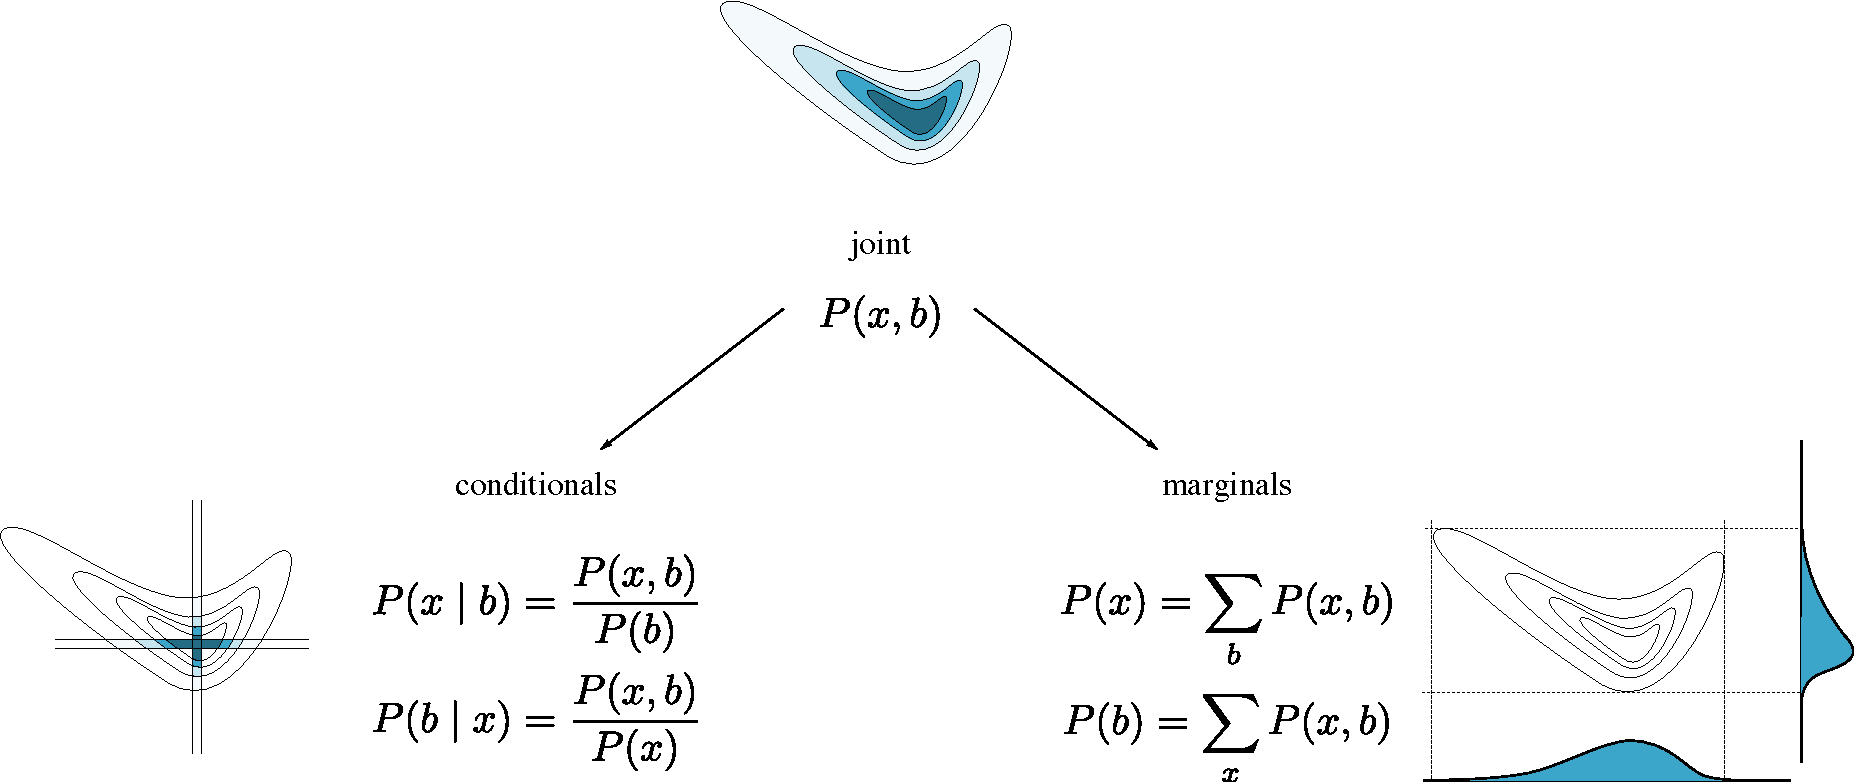
\includegraphics[width=\textwidth]{./figs/Joint-Conditional-Marginal.pdf}
\end{figure}

\subsection{Bayesian inference}
\no Prior, likelihood, posterior
\begin{itemize}
	\item Data: $D = \{x_1, x_2, \ldots x_n\}$, independent measurements.
	\item Model: $M$ with $\theta$: parameter(s) to estimate
	\item Prior: $P(\theta)$
	\item Likelihood: $P(D\;|\;\theta) = P(d_1\;|\;\theta) \;P(d_2\;|\;\theta)\;\ldots \;P(d_n\;|\;\theta) = \prod_{i=1}^n P(d_i\;|\;\theta)$
	\item Unnormalized posterior: $P^\ast(\theta\;|\;D) \;=\; P(D\;|\;\theta) \;P(\theta)$
	\item Normalization: $Z = \sum_\theta P^\ast(\theta\;|\;D)$
	\item Posterior: $P(\theta\;|\;D) = \frac{1}{Z} P^\ast(\theta\;|\;D)$
\end{itemize}
Example

``Three light bulbs of the same make lasted 1, 2 and 5 months of continuous use. Let us estimate the lifetime of this kind of light bulb.''
\begin{itemize}
	\item $D = \{t_1, t_2, t_3\} = \{1,2,5\}$
	\item $M$: Light bulbs have average lifetime of $T$ months.
	\item $P(T) = \frac{1}{1000}$, uniform on [0,1000].
	\item $P(t\;|\;T) = \frac{1}{T}\exp\left(-\frac{t}{T}\right)$
	\item $P(D\;|\;T) = \prod_i P(t_i\;|\; T) = \prod_{i=1}^3 \frac{1}{T}\exp\left(-\frac{t_i}{T}\right) = \frac{1}{T^3} \exp\left(-\frac{1 + 2 + 5}{T}\right)$
	\item $P^\ast(T\;|\;D) = \frac{1}{T^3} \exp\left(-\frac{8}{T}\right)$
	\item $Z$ and  $P(T\;|\;D)$ can be determined numerically:
\begin{lstlisting}[language=python]
import numpy as np

T_arr = np.linspace(0.1, 1000, 10_000)
Pstar_arr = 1.0/T_arr**3 * np.exp(-8/T_arr)
Z = np.sum(Pstar_arr)
P_arr = Pstar_arr / Z
\end{lstlisting}
	yielding $Z = 0.1562$
	\item $\mathbb{E}(T\;|\;D) = \sum_T T \;P(T\;|\;D)$ 
	\item $\text{std}(T\;|\;D) = \sqrt{\sum_T (T - \mathbb{E}(T))^2 \; P(T\;|\;D)}$
\begin{lstlisting}[language=python]
T_ev = np.sum(T_arr * P_arr)
T_std = np.sqrt(np.sum((T_arr - T_ev)**2 * P_arr))
\end{lstlisting}
	yielding $\mathbb{E}(T\;|\;D) = 7.937$, \quad $\text{std}(T\;|\;D) = 14.48$.
\end{itemize}


\subsection{Model comparison}
\no New definition: Evidence
\begin{itemize}
	\item Data: $D$
	\item Model 1: $M_1$ with parameter $\theta_1$ and prior $P(\theta_1\;|\; M_1)$, and likelihood $P(D\;|\;\theta_1, M_1)$
	\item Model 2: $M_2$ with parameter $\theta_2$ and prior $P(\theta_2\;|\; M_2)$, and likelihood $P(D\;|\;\theta_2, M_2)$
	\item Prior on models: $P(M_1) = 0.5$, \; $P(M_2) = 0.5$.
	\item Evidence for each model: $P(D\;|\;M_i) = \sum_\theta P(D\;|\;\theta_i, M_i) P(\theta_i\;|\;M_i)$
	\item Unnormalized posterior: $P^\ast(M_1\;|\;D) = P(D\;|\;M_1) \; P(M_1)$,\quad and $P^\ast(M_2\;|\;D) = P(D\;|\;M_2) \; P(M_2)$
	\item Normalization: $Z = P^\ast(M_1\;|\;D) + P^\ast(M_2\;|\;D)$.
\end{itemize}
Example

``Waiting for my baggage at the airport carousel, there are two possibilities: 1) It could miss the plane, and will never come, or 2) It was on the plane and it had a 1/20 chance of arriving within any of the 1-minute intervals between 0 and 20 minutes. Now, given what is the posterior probability of model 2 given that 14 minutes has passed and the bas has not arrived?''
\begin{itemize}
	\item $D = \{\text{Bag has not arrived after } t_\text{wait}=14 \text{ minutes}\}$
	\item $M_1$: It never arrives, $P(D\;|\;M_1) = 1$
	\item $M_2$: It shows up some time between 0 and 20 minutes, $P(t_\text{bag}\;|\;M_2) = 1/20$ for $t_\text{bag} \in [0, 20]$, and the likelihood is $P(D\;|\;t_\text{bag}, M_2) = 1$, if $t_\text{bag} > t_\text{wait}$, and 0 otherwise.
	\item $P(M_1) = 0.1$, \quad $P(M_2)= 0.9$
	\item $P(D\;|\;M_1)$ = 1
	\item $P(D\;|\;M_2) = \sum_{t_\text{bag}} P(D\;|\;t_\text{bag}, M_2) \;P(t_\text{bag}\;|\;M_2) = \sum_{t_\text{bag}} [t_\text{bag} > 14] \times\frac{1}{20} = \frac{20 - 14}{20}$
	\item $P^\ast(M_1\;|\;D) = 1 \times 0.1$, \quad $P^\ast(M_2\;|\;D) = \frac{20 - 14}{20}\times 0.9$
	\item $Z = 0.1 + \frac{3}{10}\times 0.9 = 0.37$
	\item $P(M_2\;|\;D) = P^\ast(M_2\;|\;D) / Z = 0.7297$.
\end{itemize}
We can also plot $P(M_2\;|\;t_\text{wait})$ for all waiting times between 0 and 20 minutes.
\begin{figure}[h]
	\centering
	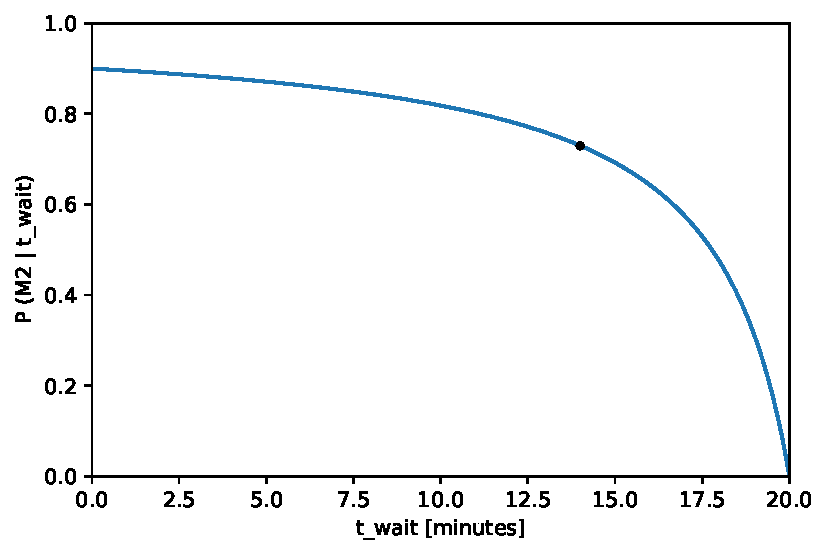
\includegraphics[width=0.5\textwidth]{figs/Baggage_wait.pdf}
\end{figure}


\subsection{Prediction}
\no New definition: Predictive distribution
\begin{itemize}
	\item Data: $D = \{x_1, x_2, \ldots x_n\}$
	\item Model: $M$ with parameter $\theta$, prior $P(\theta)$ and likelihood $P(x\;|\;\theta)$
	\item Posterior: $P(\theta\;|\;D) = P^\ast(\theta\;|\;D) / Z = \ldots$ (see previous sections)
	\item Predictive distribution: $P(X_{n+1} = x\;|\;D) = \sum_\theta P(x\;|\theta)\; P(\theta\;|\;D)$
	\item Customized prediction: $P(f(\theta)\;|\;D) = \sum_\theta f(\theta)\; P(\theta\;|\;D)$
\end{itemize}
Example

``Two player, A and B are playing a game of luck, where at the beginning of the game a ball is rolled on a pool table to divide the table in two un-equal halves: A's side and B's side. In each subsequent round, a ball is rolled. A point is given to the player on whose side the ball stops. A and B are playing this game until one of them reaches 6 points. The current score is 5 to 3 in favor of A. What is the chance that A will win this game?''
\begin{itemize}
	\item $D = \{n_A = 5, n_B = 3\}$
	\item $M$, first ball: $P(b) = 1$ in $[0,1]$
	\item $P(\text{A scores}\;|\;b) = b$
	\item $P(D\;|\;b) = \text{Binomial}(5\;|\;5 + 3, \;b)$
	\item $P^\ast(b_0\;|\;D) = \text{Binomial}(5\;|\; 8, b) \times 1$
	\item $Z = \sum_{b} \text{Binomial}(5\;|\; 8, b)$ can be calculated numerically
\begin{lstlisting}[language=python]
import numpy as np
from scipy.stats import binom

b_arr = np.linspace(0, 1, 1000)
Pstar_arr = binom.pmf(5, 8, b_arr)
Z = np.sum(Pstar_arr)
\end{lstlisting}
	\item $P(\text{A wins}\;|\;b, D) = 1 - P(\text{B wins}\;|\;b, D) = 1 - (1 - b)^3 = f(b)$
	\item $P(\text{A wins}\;|\;D) = \sum_{b} f(b) P^\ast(b\;|\;D) / Z$
\begin{lstlisting}[language=python]
P_arr = Pstar_arr / Z
P_Awins = np.sum((1 - (1 - b_arr)**3) * P_arr)
\end{lstlisting}
	yielding $P(\text{A wins}\;|\;D) = 0.909$
\end{itemize}







\newpage
\section{Maximum Likelihood Estimate and Exact inference}

The one-size-fits-all method of inferring unknown model parameters is called ``Maximum Likelihood Estimate''. It is calculated by finding the parameter values that maximize the generative probability of the observed data.

\subsection{Maximum likelihood estimate}
\no MLE-method
\begin{itemize}
	\item We record a series of measurements, $D = \{x_1, x_2, \ldots x_N\}$.
	\item We construct a model that specifies the probability of each data point $x_i$, $P(x_i\;|\;\theta)$, as a function of model parameter(s) $\theta$, the value(s) of which we wish to infer.
	\item The sum of the log probability term yields the log likelihood \emph{of the parameter}, \\
	\be
		L(\theta) := \log P(D\;|\;\theta) = \log \prod_{i=1}^N P(D\;|\; \theta) = \sum_{i=1}^N \log P(x_i\;|\;\theta)
	\ee
	\item Optimizing the value of $\theta$ to get to the maximum of $L$ yields the MLE of $\theta$: 
	\be
		\theta_\text{MLE} = \text{argmax}_{\theta} L(\theta),
	\ee
	This can be done either
	\begin{itemize}
		\item {\bf numerically}, by gradient descent or EM methods (see section \ref{sec:EM}), or
		\item {\bf analytically}, by setting the first derivatives to 0, and solving the resulting system of equations.
	\end{itemize}
		
\end{itemize}

\no {\bf Example 1: Normal model} (analytical MLE)
\begin{itemize}
	\item We observe a collection of real values $D = \{x_i \in \mathds{R}\}_{i=1}^N$
	\item The normal model has two parameters,  $\mu \in \mathds{R}$, and  $\sigma^2 > 0$, which define the probability density of each data point as
	\be
		P(x_i\;|\;\mu, \sigma^2) = \text{Normal}(x_i\;|\;\mu, \sigma^2) = \frac{1}{\sqrt{2\pi \sigma^2}}\exp\left[-\frac{(x_i - \mu)^2}{2\sigma^2}\right].
	\ee
	\item The log likelihood of the model parameters is
	\ba
		L(\mu, \sigma^2) 
		&=& \sum_{i=1}^N \log \left(\text{Normal} (x_i\;|\; \mu, \sigma^2)\right) = - \frac{N}{2}\log(\sigma^2) - \sum_{i=1}^N \frac{(x_i - \mu)^2}{2\sigma^2} + \text{const.}
	\ea
	\item To calculate the formulas for the analytical MLE of $\mu$ and $\sigma^2$, we calculate the first order partial derivatives of $L$, and set them to zero. (With $[\ldots]_\text{MLE}$ with denote that the enclosed formula is evaluated at the MLE point, $(\mu_\text{MLE}, (\sigma^2)_\text{MLE})$.)
		\ba
			0 &=& \left[\frac{\partial L}{\partial \mu}\right]_\text{MLE} = \left[\sum_{i=1}^N\frac{\mu - x_i}{\sigma^2}\right]_\text{MLE} \qquad \hspace{2.2cm}\Rightarrow \qquad \mu_\text{MLE} = \frac{1}{N}\sum_{i=1}^N x_i.
			\\
			0 &=& \left[\frac{\partial L}{\partial (\sigma^2)}\right]_\text{MLE} = \left[-\frac{N}{2\sigma^2} + \sum_{i=1}^N \frac{(x_i-\mu)^2}{2(\sigma^2)^2}\right]_\text{MLE}\qquad \Rightarrow \qquad (\sigma^2)_\text{MLE} = \frac{1}{N} \sum_{i=1}^N (x_i - \mu_\text{MLE})^2
		\ea
\end{itemize}
This result shows that the empirical mean and empirical variance (the right hand sides of the equations above) are exactly the MLE estimates of $\mu$ and $\sigma^2$, respectively.


\newpage
\no {\bf Example 2: Cauchy distribution} (numerical MLE)
\begin{itemize}
	\item Let's say we observe the following five data point $D = \{-10, 1, 2, 5, 20\}$, and
	\item we wish to fit a Cauchy distribution to this data, parameterized by $m \in \mathds{R}$ and $s > 0$.
	\be
		P(x_i\;|\;m, s) = \text{Cauchy}(x_i\;|\;m, s) = \frac{1}{s \pi} \frac{1}{1 + \left[(x_i - m)/s\right]^2}
	\ee
	\item The log likelihood of the model parameters is
		\be
			L(m, s) = \sum_{i=1}^N \log \text{Cauchy}(x_i\;|\;m, s) = -N\log(s) - \sum_{i=1}^N\log\!\left(1 + \left[\frac{x_i - m}{s}\right]^2\right) + \text{const.}
		\ee

	\item Since there is no closed-form solution, we us numerical maximization to find $m_\text{MLE}$ and $s_\text{MLE}$. The following python code uses \texttt{scipy.optimize.minimize()} to find the local maximum near the initial starting point, $m_0 = 0$, $s_0 = 10$.
\begin{lstlisting}[language=python]
import numpy as np
from scipy.optimize import minimize

def cauchy_total_log_likelihood(X, m, s):
    X = np.array(X)
    
    L = 0
    L += -len(X)/2 * np.log(s**2)
    L += -np.sum( np.log(1 + (X - m)**2 / s**2 ) )
    
    return L

X = [-10, 1, 2, 5, 20]
def func_to_minimize(theta):
    m = theta[0]
    s = theta[1]
    return  - cauchy_total_log_likelihood(X, m, s)

m0 = 0
s0 = 10
result = minimize(func_to_minimize, [m0, s0])
m_MLE, s_MLE = result.x
\end{lstlisting}
	\item This yields $m_\text{MLE} = 2.251, \; s_\text{MLE} = 3.090$. Here is the corresponding Cauchy probability density:
		\begin{figure}[h]
			\centering
			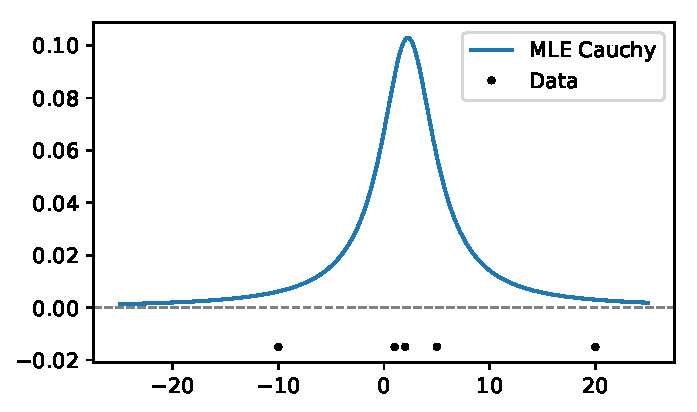
\includegraphics[width=0.44\textwidth]{./figs/Cauchy_MLE.pdf}
		\end{figure}
\end{itemize}


\newpage
\subsection{Exact inference examples}

A very small number of models can be inferred exactly. This means, we can derive closed form solutions for the posterior distribution of their parameters. Consequently the posterior function and various summary statistics (e.g. mean and standard deviation) of the model parameter can be calculated exactly and efficiently.
\\

\no {\bf Binomial model}
\begin{itemize}
	\item We record the number of successes $k_i$ in each of the $i = 1,\ldots N$ experimental runs ($N=1$ is also possible), each of which contains $n_i$ attempts. The data we collect is $D = \{(k_1, n_1), (k_2, n_2), \ldots, (k_N, n_N)\}$, where $0 \leq k_i \leq n_i$, positive integers. 
	\item (Note: The resulting formulas will show that it is enough to know the total number of successes $k_\text{tot}$ and total number of attempts $n_\text{tot}$, if the same binomial model is responsible for all experimental runs.)
	\item If each attempt is independent of the others, then the binomial model is justified, and the corresponding probability for a single experiment can be written as
	\be
		P(k_i \;|\; n_i, p) = \text{Binomial} (k_i\;|\;n_i, p) = {n_i \choose k_i} \; p^{k_i} (1-p)^{n_i - k_i}
	\ee
	which is a function of the success probability $p$, $0 \leq p \leq $, for which we assume a flat prior density: $P(p) = 1$, on the $[0,1]$ interval.
	\item The posterior of $p$, after considering all experimental runs, can be recognized as a beta distribution:
	\ba 
		P(p\;|\;D)
		&=& \frac{1}{Z} \prod_{i=1}^N \left[p^{k_i} (1-p)^{n_i - k_i}\right] = \frac{1}{Z} p^{k_\text{tot}} (1 - p)^{n_\text{tot} - k_\text{tot}} 
		\\
		&=& \frac{\Gamma(\alpha + \beta)}{\Gamma(\alpha)\Gamma(\beta)} p^{\alpha-1} (1-p)^{\beta-1} = \text{Beta}(p\;|\;\alpha = k_\text{tot} + 1,\beta = n_\text{tot} - k_\text{tot} +1),
	\ea
	where $k_\text{tot} = \sum_i k_i$ and $n_\text{tot} = \sum_i n_i$. Using the known formulas of the beta distribution, we can write the mean, mode and standard deviation of $p$ as 
	\ba
		&& \mathbb{E}(p) = \frac{\alpha}{\alpha + \beta} = \frac{k_\text{tot} + 1}{n_\text{tot} + 2}, 
		\quad 
		\text{mode}(p) = \frac{\alpha - 1}{\alpha + \beta -2} = \frac{k_\text{tot}}{n_\text{tot}},
		\\ 
		&& \text{std}(p) = \frac{\sqrt{\alpha \beta}}{(\alpha + \beta) \sqrt{\alpha + \beta + 1}} = \frac{\sqrt{(k_\text{tot} + 1)(n_\text{tot} - k_\text{tot} + 1)}}{(n_\text{tot} + 2)\sqrt{n_\text{tot} + 3}}
	\ea
	\item Note: The mode of the posterior (calculated under flat prior) coincides with the maximum likelihood estimate, $p_\text{MLE} = k_\text{tot} / n_\text{tot}$.
\end{itemize}
\vspace{0.5cm}

\no {\bf Poisson model}
\begin{itemize}
	\item Within each of the $i=1,\ldots N$ measurement windows, we observe $k_i$ number of events. The collected data is $D = \{k_1, k_2, \ldots k_N\}$, where $k_i \geq 0$, positive integers.
	\item (Note: The formula of the posterior will show that knowing the total number of events $k_\text{tot}$ and the number of windows $N$ is enough.)
	\item The Poisson model for a single measurement window prescribes the probability 
	\be
		P(k_i\;|\;\lambda) = \text{Poisson}(k\;|\;\lambda) = e^{-\lambda} \frac{\lambda^{k_i}}{k_i!},
	\ee 
	where $\lambda > 0$ is the ``typical number of observations'', for which we assume a flat (and improper) prior: $P(\lambda) = \text{const.}$
	\item The posterior of $\lambda$ turns out to be a gamma distribution:
	\ba
		P(\lambda\;|\;D) 
		&=& \frac{1}{Z} \prod_{i=1}^N\left[e^{-\lambda} \lambda^{k_i}\right] = \frac{1}{Z} e^{-N\lambda} \lambda^{k_\text{tot}}
		= \frac{\beta^\alpha}{\Gamma(\alpha)} \lambda^{\alpha -1} e^{-\beta\lambda} = \text{Gamma}(\lambda\;|\; \alpha = k_\text{tot} + 1, \beta = N),
	\ea
	where $k_\text{tot} = \sum_i k_i$. Using the known formulas for the gamma distribution, the mean, mode and standard deviation of $\lambda$ can be written as
	\ba
		\mathbb{E}(\lambda) = \frac{\alpha}{\beta} = \frac{k_\text{tot} + 1}{N},\quad \text{mode}(\lambda) = \frac{\alpha - 1}{\beta} = \frac{k_\text{tot}}{N},\quad
		\text{std}(\lambda) = \frac{\sqrt{\alpha}}{\beta} = \frac{\sqrt{k_\text{tot} + 1}}{N}
	\ea
	\item Note: The mode of the posterior (calculated under flat prior) coincides with the maximum likelihood estimate, $\lambda_\text{MLE} = k_\text{tot} / N$.
\end{itemize}
\vspace{0.5cm}

\no {\bf Multinomial model}
\begin{itemize}
	\item Similarly to the binomial model, we perform a series of experimental runs, $i = 1,\ldots N$, each consisting some number of attempts, each of which can result in $M$ different outcomes. For the $i$th experimental run the collected data is $D_i = (k_{i,1}, k_{i,2}, \ldots k_{i,M})$, where $k_{i,j} \geq 0$ is the number of times outcome $j$ was found in experiment $i$. The complete observed data is $D = \{D_1, D_2, \ldots D_N\}$.
	\item (Note: The formulas for the posterior will show that it is enough to know the number of each outcomes aggregated across all runs, $k_{\text{tot}, j}$, if the same multinomial process is responsible for all runs.)
	\item The multinomial model (which is justified if the attempts are independent from each other) prescribes the probability for the outcome vector $\{k_{i,j}\}_{j=1}^M$ of one experiment
	\be
		P(\{k_{i,j}\}_{j=1}^M\;|\;p) = \text{Multinomial}(\{k_{i,j}\}_{j=1}^M\;|\;p) = k_{i,\text{tot}}! \prod_j \frac{p_j^{k_{i,j}}}{k_{i,j}!},
	\ee
	where each element of the probability vector $p = (p_1, p_2, \ldots p_M)$, $0 \leq p_j \leq 1$ is the probability of outcome $j$. Since one of the outcomes is certain to happen, $\sum_j p_j = 1$. We assume a flat prior for the probability vector $P(p) = \text{const.}$ (on the $M-1$ dimensional unit simplex).
	\item The posterior of $p$, after considering all runs, can be written as a Dirichlet distribution:
	\ba
		P(p\;|\;D) &=& \frac{1}{Z} \prod_{i=1}^N \prod_{j=1}^M (p_j)^{k_{i,j}} = \frac{1}{Z} \prod_{j=1}^{M} (p_j)^{k_{\text{tot}, j}} = \Gamma(\alpha_\text{tot}) \prod_{j=1}^M \frac{(p_j)^{\alpha_j - 1}}{\Gamma(\alpha_j)} = \text{Dirichlet}(p\;|\;\alpha_j = k_{\text{tot}, j} + 1),
	\ea
	where $k_{\text{tot}, j} = \sum_i k_{i,j}$, and $\alpha_\text{tot} = \sum_j \alpha_j = k_\text{tot,tot} + M$. Mean, mode and marginal standard deviation are
	\ba
		&& \mathbb{E}(p_j) = \frac{\alpha_j}{\alpha_\text{tot}} = \frac{k_{\text{tot},j} + 1}{k_\text{tot,tot} + M},
		\quad
		\text{mode}(p):\; p_j = \frac{\alpha_j-1}{\alpha_\text{tot}-M} = \frac{k_{\text{tot},j}}{k_\text{tot,tot}}
		\\
		&& \text{std}(p_j) = \frac{\sqrt{\alpha_j(\alpha_\text{tot} - \alpha_j)}}{\alpha_\text{tot}\sqrt{\alpha_\text{tot} + 1}} = \frac{\sqrt{(k_{\text{tot},j} + 1) (k_{\text{tot,tot}} - k_{\text{tot},j} + M - 1)}} {(k_{\text{tot,tot}} + M) \sqrt{k_{\text{tot,tot}} + M + 1}}
	\ea
	\item Note: The mode of the posterior (calculated under flat prior) coincides with the maximum likelihood estimate, $p_{\text{MLE},j} = k_{\text{tot},j} / k_\text{tot,tot}$.
\end{itemize}
\vspace{0.5cm}

\newpage
\no {\bf Exponential model}
\begin{itemize}
	\item We observe a sequence of events, $i = 1,\ldots N$. We record the waiting times $t_i$ between event $i-1$ and event $i$ ($t_1$ is the waiting time from the start of observation until the first event). The data is $D = \{t_1, t_2, \ldots t_N\}$, where $t_i > 0$.
	\item (Note: The formula for the posterior will show that, if the events are generated by a Poisson process, then it is enough to know the total elapsed time $t_\text{tot}$ and the number of events $N$.)
	\item If the events are generated by a Poisson process (i.e. they are independent from each other and the elapsed time), then the waiting times are exponentially distributed:
	\be
		P(t_i\;|\;\gamma) = \text{Exponential}(t_i\;|\;\gamma) = \gamma e^{-\gamma t_i},
	\ee
	where $\gamma > 0$ is the rate of events, for which we assume a flat (and improper) prior: $P(\gamma) = \text{const.}$
	\item The posterior of $\gamma$ can be written as a gamma distribution:
	\ba
		P(\gamma\;|\;D) &=& \frac{1}{Z} \prod_{i=1}^N \left[\gamma e^{-\gamma t_i}\right] = \frac{1}{Z} \gamma^N e^{-\gamma t_\text{tot}} = \frac{\beta^\alpha}{\Gamma(\alpha)} \gamma^{\alpha-1} e^{-\beta\gamma} = \text{Gamma}(\gamma\;|\;\alpha = N+1, \beta = t_\text{tot}),
	\ea
	where $t_\text{tot} = \sum_i t_i$. Using the known formulas for the gamma distribution, we can write the mean, mode, standard deviation of $\gamma$ as 
	\be
		\mathbb{E}(\gamma) = \frac{\alpha}{\beta} = \frac{N+1}{t_\text{tot}},\quad \text{mode}(\gamma) = \frac{\alpha -1}{\beta} = \frac{N}{t_\text{tot}}, \quad\text{std}(\gamma) = \frac{\sqrt{\alpha}}{\beta} = \frac{\sqrt{N+1}}{t_\text{tot}}
	\ee
	\item Note: The mode of the posterior (calculated under flat prior) coincides with the maximum likelihood estimate, $\gamma_\text{MLE} = N / t_\text{tot}$.
	\item Note: The result is meaningful even for $N=0$, which corresponds to a $t_\text{tot}$-long measurement session during which no event was observed. This results in a posterior which is identical to an exponential distribution: $P(\gamma\;|\;D) = \text{Gamma}(\gamma\;|\;\alpha = 1, \;\beta = t_\text{tot}) = t_\text{tot} e^{-t_\text{tot} \gamma} = \text{Exponential}(\gamma\;|\;t_\text{tot})$.
\end{itemize}
\vspace{0.5cm}


\no {\bf Normal}
\begin{itemize}
	\item We observe one-dimensional data points $D = \{x_1, x_2, \ldots x_N\}$, where $x \in \mathds{R}$.
	\item The normal model prescribes the following probability for each data point:
	\be
		P(x_i\;|\;\mu, \sigma^2) = \text{Normal}(x_i\;|\;\mu, \sigma^2) = \frac{1}{\sqrt{2\pi \sigma^2}} \exp\!\left[-\frac{(x_i - \mu)^2}{2\sigma^2}\right],
	\ee
	as a function of $\mu$ (expected value) $\in \mathds{R}$, and $\sigma^2$ (variance) $ >0$, for which we assume a flat (and improper) priors: $P(\mu, \sigma^2) = \text{const.}$
	\item With the notations, $m = \frac{1}{N}\sum_i x_i$ being the empirical mean, $s^2 = \frac{1}{N}\sum_i (x_i - m)^2$ being the empirical variance, the joint posterior of $\mu, \sigma^2$ can be written as
	\ba
		P(\mu, \sigma^2\;|\;D) 
		&=& \frac{1}{Z}\prod_{i=1}^N \left\{\frac{1}{\sqrt{\sigma^2}} \exp\!\left[-\frac{(x_i-\mu)^2}{2\sigma^2}\right]\right\} = \frac{1}{Z} \left(\frac{1}{\sigma^2}\right)^{N/2} \exp\!\left[-\frac{Ns^2 + N(\mu - m)^2}{2\sigma^2}\right]
		\\
		&=&
		\frac{\sqrt{\lambda}}{\sqrt{2\pi \sigma^2}}\frac{\beta^\alpha}{\Gamma(\alpha)} \left(\frac{1}{\sigma^2}\right)^{\alpha + 1} \exp\!\left[-\frac{2\beta + \lambda(\mu - \mu_c)^2}{2\sigma^2}\right]
		\\
		&=& \text{Normal-Inverse-Gamma}\Big(\mu, \sigma^2\;\Big|\; \alpha = \frac{N-3}{2},\; \beta = \frac{Ns^2}{2},\; \mu_c = m,\; \lambda=N\Big).
	\ea
	This is a two-dimensional joint distribution, the mode of which is at
	\be
		\text{mode}(\mu, \sigma^2) = (m, s^2).
	\ee
	
	\item Integrating out $\sigma^2$ results in the marginal distribution of $\mu$:
	\ba
		P(\mu\;|\;D) 
		&=& \sum_{\sigma^2} P(\mu, \sigma^2\;|\;D) = \frac{\Gamma\left(\frac{N-2}{2}\right)}{\Gamma\left(\frac{N-3}{2}\right)} \frac{1}{\sqrt{\pi s^2}}\left[1 + \frac{(\mu - m)^2}{s^2}\right]^{-(N-2)/2}
		\\
		&=& \frac{\Gamma\left(\frac{\nu + 1}{2}\right)}{\Gamma\left(\frac{\nu}{2}\right)} \frac{1}{\sqrt{\pi \nu}}\left[1 + \frac{1}{\nu}\left(\frac{\mu - \text{loc}}{\text{scale}}\right)^2\right]^{-(\nu+1)/2} \frac{1}{\text{scale}} 
		\\ 
		&=& \text{t-distr}\Big(\mu\;\Big|\;\text{loc}=m,\; \text{scale}=\frac{s}{\sqrt{N-3}},\; \nu=N-3\Big),
	\ea
	where $\nu$ is the ``degrees of freedom'' of the Student's t distribution. 
	Using the known formulas for the shifted and scaled Student's t distribution, we can write the mean, \emph{marginal} mode and standard deviation of $\mu$ as
	\be
		\mathbb{E}(\mu) = m,\quad \text{mode}(\mu) = m,\quad \text{std}(\mu) = \frac{s}{\sqrt{N-3}} \sqrt{\frac{\nu}{\nu-2}} = \frac{s}{\sqrt{N-5}},
	\ee

	\item Integrating out $\mu$ results in the marginal distribution of $\sigma^2$:
	\ba
		P(\sigma^2\;|\;D) &=& \sum_\mu P(\mu, \sigma^2\;|\;D) = \frac{\beta^\alpha}{\Gamma(\alpha)}\left(\frac{1}{\sigma^2}\right)^{\alpha+1} \exp\left(-\frac{\beta}{\sigma^2}\right)
		\\
		&=& \text{Inverse-Gamma}\Big(\sigma^2\;\Big|\;\alpha = \frac{N-3}{2},\;\beta = \frac{Ns^2}{2}\Big)
	\ea
	Using the known formulas for the inverse gamma distribution, we can write the mean, \emph{marginal} mode and standard deviation of $\sigma^2$ as
	\ba
		&& \mathbb{E}(\sigma^2) = \frac{\beta}{\alpha - 1} = s^2 \frac{N}{N-5},\quad \text{mode}(\sigma^2) = \frac{\beta}{\alpha + 1} = s^2\frac{N}{N-1} \\
		&& \text{std}(\sigma^2) = \frac{\beta}{(\alpha-1)\sqrt{\alpha-2}} = s^2\frac{\sqrt{2} N}{(N-5)\sqrt{N-7}}
	\ea

	\item Note: While the mean and the standard deviation are unaffected by marginalization, the mode, in general, depends on whether we evaluate it on the joint distribution  $P(\mu, \sigma^2\;|\;D)$ or on the marginals $P(\mu\;|\;D)$ and $P(\sigma^2\;|\;D)$.  With the assumption of the flat prior, the mode of $\mu$ happens to be the same both in the joint in and the marginal, and it coincides with its maximum likelihood estimate. 
	\be
		[\text{mode}(\mu, \sigma^2)]_1 = \text{mode}(\mu) = m = \frac{1}{N} \sum_{i=1}^N x_i= \mu_\text{MLE}
	\ee
	With the assumption of flat prior, the mode of $\sigma^2$ in the joint is identical to its maximum likelihood estimate, while the mode of the $\sigma^2$ marginal coincides with the widely-used unbiased estimator of $\sigma^2$.
	\ba
		[\text{mode}(\mu, \sigma^2)]_2 = s^2 = \frac{1}{N} \sum_{i=1}^N (x_i - m)^2 = (\sigma^2)_\text{MLE}& \neq & \text{mode}(\sigma^2) = s^2\frac{N}{N-1} = \frac{1}{N-1} \sum_{i=1}^N (x_i - m)^2
	\ea
\end{itemize}

\vspace{0.5cm}

The next page shows a graphical summary of the exactly-solvable models discussed above. The left column features a typical distribution the model prescribes for the data. The right column shows a typical posterior probability density for the model parameters.

\newpage
\begin{figure}[!]
	\centering
	\includegraphics[width=\textwidth]{./figs/Exact-Inference-summary.pdf}
\end{figure}


\newpage
\newpage
\section{Priors, Regularization, AIC, BIC, LRT}


\subsection{Improper and proper priors}
\no Improper priors are not normalizable, i.e. $\sum_\theta P(\theta) = \infty$
\begin{itemize}
	\item Flat prior: $P(\theta) = \text{const.}$ over any infinite domain.
	\item Uninformative priors (from transformation invariance or max-entropy principles)
	\begin{itemize}
		\item Location parameter: $P(m) = \text{const.}$, on $m \in (-\infty, +\infty)$,
		\item Scale parameter: $P(s) = \frac{\text{const.}}{s}$, on $s\in (0, \infty)$,
		\item Probability parameter: $P(p) = \frac{\text{const.}}{p(1-p)}$, on $p\in(0,1)$.
	\end{itemize}
\end{itemize}
Proper priors are normalized, i.e. $\sum_\theta P(\theta) = 1$.

\subsection{Regularization}
\no Regularized model training
\begin{itemize}
	\item Data: $D$, 
	\item Model: $M$ with parameters $\theta$, likelihood $P(D\;|\;\theta)$
	\item Cost function $= - \log P(D\;|\;\theta) = - L(\theta)$, the log likelihood
	\item Penalty: $\text{penalty}(\theta)$, which is high for implausible $\theta$ values.
	\item Regularized optimum: $\theta_\text{reg.opt.} = \text{arg min}_\theta (-L(\theta) + \text{penalty}(\theta))$
\end{itemize}

\subsection{Linear regression}
\begin{itemize}
	\item Data: $D = \{\;(\{x_{i,k}\}_{k=1}^K, \;y_i)\;\}_{i=1}^N$, where $x_i$ (feature vector) $\in \mathds{R}^K$,  $y_i$ (predicted variable) $\in \mathds{R}$.
	\item Parameters: $\{b_k\}_{k=1}^K$, where $b_k$ (coefficient or weight) $\in \mathds{R}$.
	\item Model:
		\ba
			y_i &=& \sum_{k=1}^K x_{i,k} b_k + \varepsilon_i, \quad \text{with}\quad P(\varepsilon_i) = \text{Normal}(\varepsilon_i\;|\; \mu = 0, \sigma^2 = \sigma^2) \\
			y &=& X b + \varepsilon \\
			&& \text{or equivalently} \\
			P(y\;|\;X, b) &=& \prod_{i=1}^N\text{Normal}\left(y_i\;\big|\;\mu = (X b)_i, \;\sigma^2=\sigma^2\right)
		\ea
	\item Log likelihood: $L(b) = \log P(y\;|\;X, b) = -\frac{N}{2}\log(\sigma^2) - \frac{1}{2\sigma^2} \sum_{i=1}^N \Big[y_i - \sum_{k} x_{i,k} b_k\Big]^2$
	\item Maximum likelihood estimate: $b_\text{MLE} = \text{arg max}_b\; L(b) = (X^\top X)^{-1} X^\top y$, \quad $(\sigma^2)_\text{MLE} = \frac{1}{N}|| y - Xb ||^2$
	\item Regularization:
	\begin{itemize}
		\item ``L1 regularization'': $\text{penalty}(b) = \alpha_1 \sum_k |b_k|$ \\ 
		\quad $\Leftrightarrow$ \quad Laplace prior: $P(b_k) = \text{const.} \times e^{- \alpha_1|b_k|} = \text{Laplace}(b_k\;|\;\text{loc}=0, \text{scale}=1/\alpha_1)$

		\item ``L2 regularization'': $\text{penalty}(b) = \frac{\alpha_2}{2}\sum_k (b_k)^2$ 
		\\ 
		\quad $\Leftrightarrow$ \quad Normal prior: $P(b_k) = \text{const.} \times e^{- \alpha_2(b_k)^2 / 2} = \text{Normal}(b_k\;|\;\mu=0, \sigma^2=1/\alpha_2)$

		\item ``Elastic net regularization'': $\text{penalty}(b) = \alpha_1 \sum_k |b_k| + \frac{\alpha_2}{2}\sum_k (b_k)^2$
	\end{itemize}
	The ``hyperparameters'' $\alpha_1$ and $\alpha_2$ can be optimized using ``Leave-one-out'' or ``M-fold''cross-validation.
\end{itemize}

\subsection{Model comparison with asymptotic metrics}
\no Maximum likelihood results from two models
\begin{itemize}
	\item Data $D = \{x_i\}_{i=1}^N$
	\item Null model: \hspace{6.5mm} $M_0$ with parameters $\theta_0$, and $L_0(\theta_0) = P(D\;|\;\theta_0, M_0)$, \;$\theta_{0, \text{MLE}} = \text{argmax}_{\theta_0} L_0(\theta_0)$
	\item Alternate model: $M_1$ with parameters $\theta_1$, and $L_1(\theta_1) = P(D\;|\;\theta_1, M_1)$, \;$\theta_{1, \text{MLE}} = \text{argmax}_{\theta_1} L_1(\theta_1)$
\end{itemize}
Akaike Information Criterion (AIC)
\begin{itemize}
	\item $\text{AIC}(M_i) = -2\Big[L_i(\theta_{i,\text{MLE}}) - \text{dim}(\theta_i)\Big]$ for both $i=0, 1$ models.
	\item If $\text{AIC}(M_1) < \text{AIC}(M_0)$, then $M_1$  is more plausible.
\end{itemize}
Bayesian Information Criterion (BIC)
\begin{itemize}
	\item $\text{BIC}(M_i) = -2\left[L_i(\theta_{i,\text{MLE}}) - \frac{\ln(N)}{2}\text{dim}(\theta_i)\right]$ for both $i=0, 1$ models.
	\item If $\text{BIC}(M_1) < \text{BIC}(M_0)$, then $M_1$  is more plausible.
\end{itemize}
Likelihood Ratio Test (LRT)
\begin{itemize}
	\item $\text{logLR} = \log\frac{P(D\;|\;M_1, \theta_{1,\text{MLE}})}{P(D\;|\;M_0, \theta_{0,\text{MLE}})} = L_1(\theta_{1,\text{MLE}}) - L_0(\theta_{0,\text{MLE}})$
	\item $\text{LRT pvalue} = 1 - \text{cdf }\chi^2\Big(2\,\text{logRL}\;\Big|\;\text{dof} = \text{dim}(\theta_1) - \text{dim}(\theta_0)\Big)$, where $\text{cdf }\chi^2(\ldots\;|\;\text{dof}=d)$ is the cumulative distribution function of the $\chi^2$ distribution with degrees of freedom $d$.
\end{itemize}
Model evidence
\begin{itemize}
	\item $P(D\;|\;M_i) = \sum_{\theta_i} P(D\;|\;\theta_i, M_i) \approx \exp\left(-\frac{1}{2} \text{ IC}\right)$, 
	\item where IC can be either AIC or BIC (or WAIC, WBIC)
	\item Under uniform prior (i.e. $P(M_0) = P(M_1)$), the posterior probability of the alternate model being correct is
		\be
			 P(M_1\;|\;D) \approx \frac{\exp\left(-\frac{1}{2} \text{ IC}_1\right)}{\exp\left(-\frac{1}{2} \text{ IC}_0\right) + \exp\left(-\frac{1}{2} \text{ IC}_1\right)}
		\ee
\end{itemize}

\newpage
\subsection{Example: Linear regression}
\begin{itemize}
	\item Data: $D = \{(x_i, y_i)\}_{i=1}^N$ (generated from $y = 1 - 3x - x^2/2 + x^3 + \varepsilon$ with $\text{std}(\varepsilon) = 2$).
\begin{lstlisting}[language=python]
import numpy as np
from numpy.polynomial.polynomial import polyval
from scipy.stats import norm

c_true = [1, -3, -0.5, 1]
sigma_true = 2
x_data = np.linspace(-3, 3, 20)
y_data = [polyval(x, c_true) + norm.rvs(loc=0, scale=sigma_true) 
          for x in x_data]
\end{lstlisting}
	\begin{figure}[h]
		\centering
		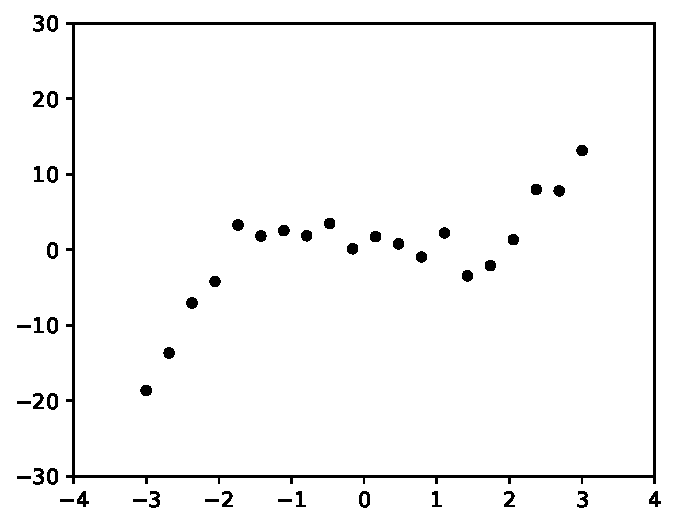
\includegraphics[width=0.4\textwidth]{./figs/03-linear-regression-data.pdf}
	\end{figure}
	\item Models: $M_K:\;K=0,1,2,\ldots$-degree polynomial, parameters: $c = (c_0, c_1, \ldots c_K)$.
	\item ``Linear features'': $X_i := (1, x_i, (x_i)^2, (x_i)^3),\ldots (x_i)^K)$.
\begin{lstlisting}[language=python]
def generate_polynomial_features(x_data, degree):
    K = degree
    N = len(x_data)
    X = np.zeros([N, K+1])
    for i, x in enumerate(x_data):
        for k in range(0, K+1, 1):
            X[i,k] = x**k
    return X
\end{lstlisting}

	\item Likelihood:
	$y = \sum_{k=0}^K X_{i,k} c_k  + \varepsilon$, with $P(\varepsilon) = \text{Normal}(\varepsilon \;|\; 0, \sigma^2)$
\begin{lstlisting}[language=python]
def log_likelihood(X, y, c, sigma2):
    N = len(y_data)
    log_like = 0
    log_like += - N/2.0 * np.log(sigma2)
    log_like += - 1.0/(2 * sigma2) * vector_norm(y - X.dot(c))**2
    return log_like
\end{lstlisting}

\newpage
	\item MLE solution: $c_\text{MLE}= (X^\top X)^{-1} X^\top y$, \quad $(\sigma^2)_\text{MLE} = \frac{1}{N}||y - X c_\text{MLE}||^2$
\begin{lstlisting}[language=python]
def fit_MLE_ploynomial(X, y):
    c_MLE = inv(X.T.dot(X)).dot(X.T).dot(y_data)
    sigma2_MLE = 1.0/len(y) * vector_norm(y - X.dot(c_MLE))**2
    return c_MLE, sigma2_MLE
\end{lstlisting}
	\begin{figure}[h]
		\centering
		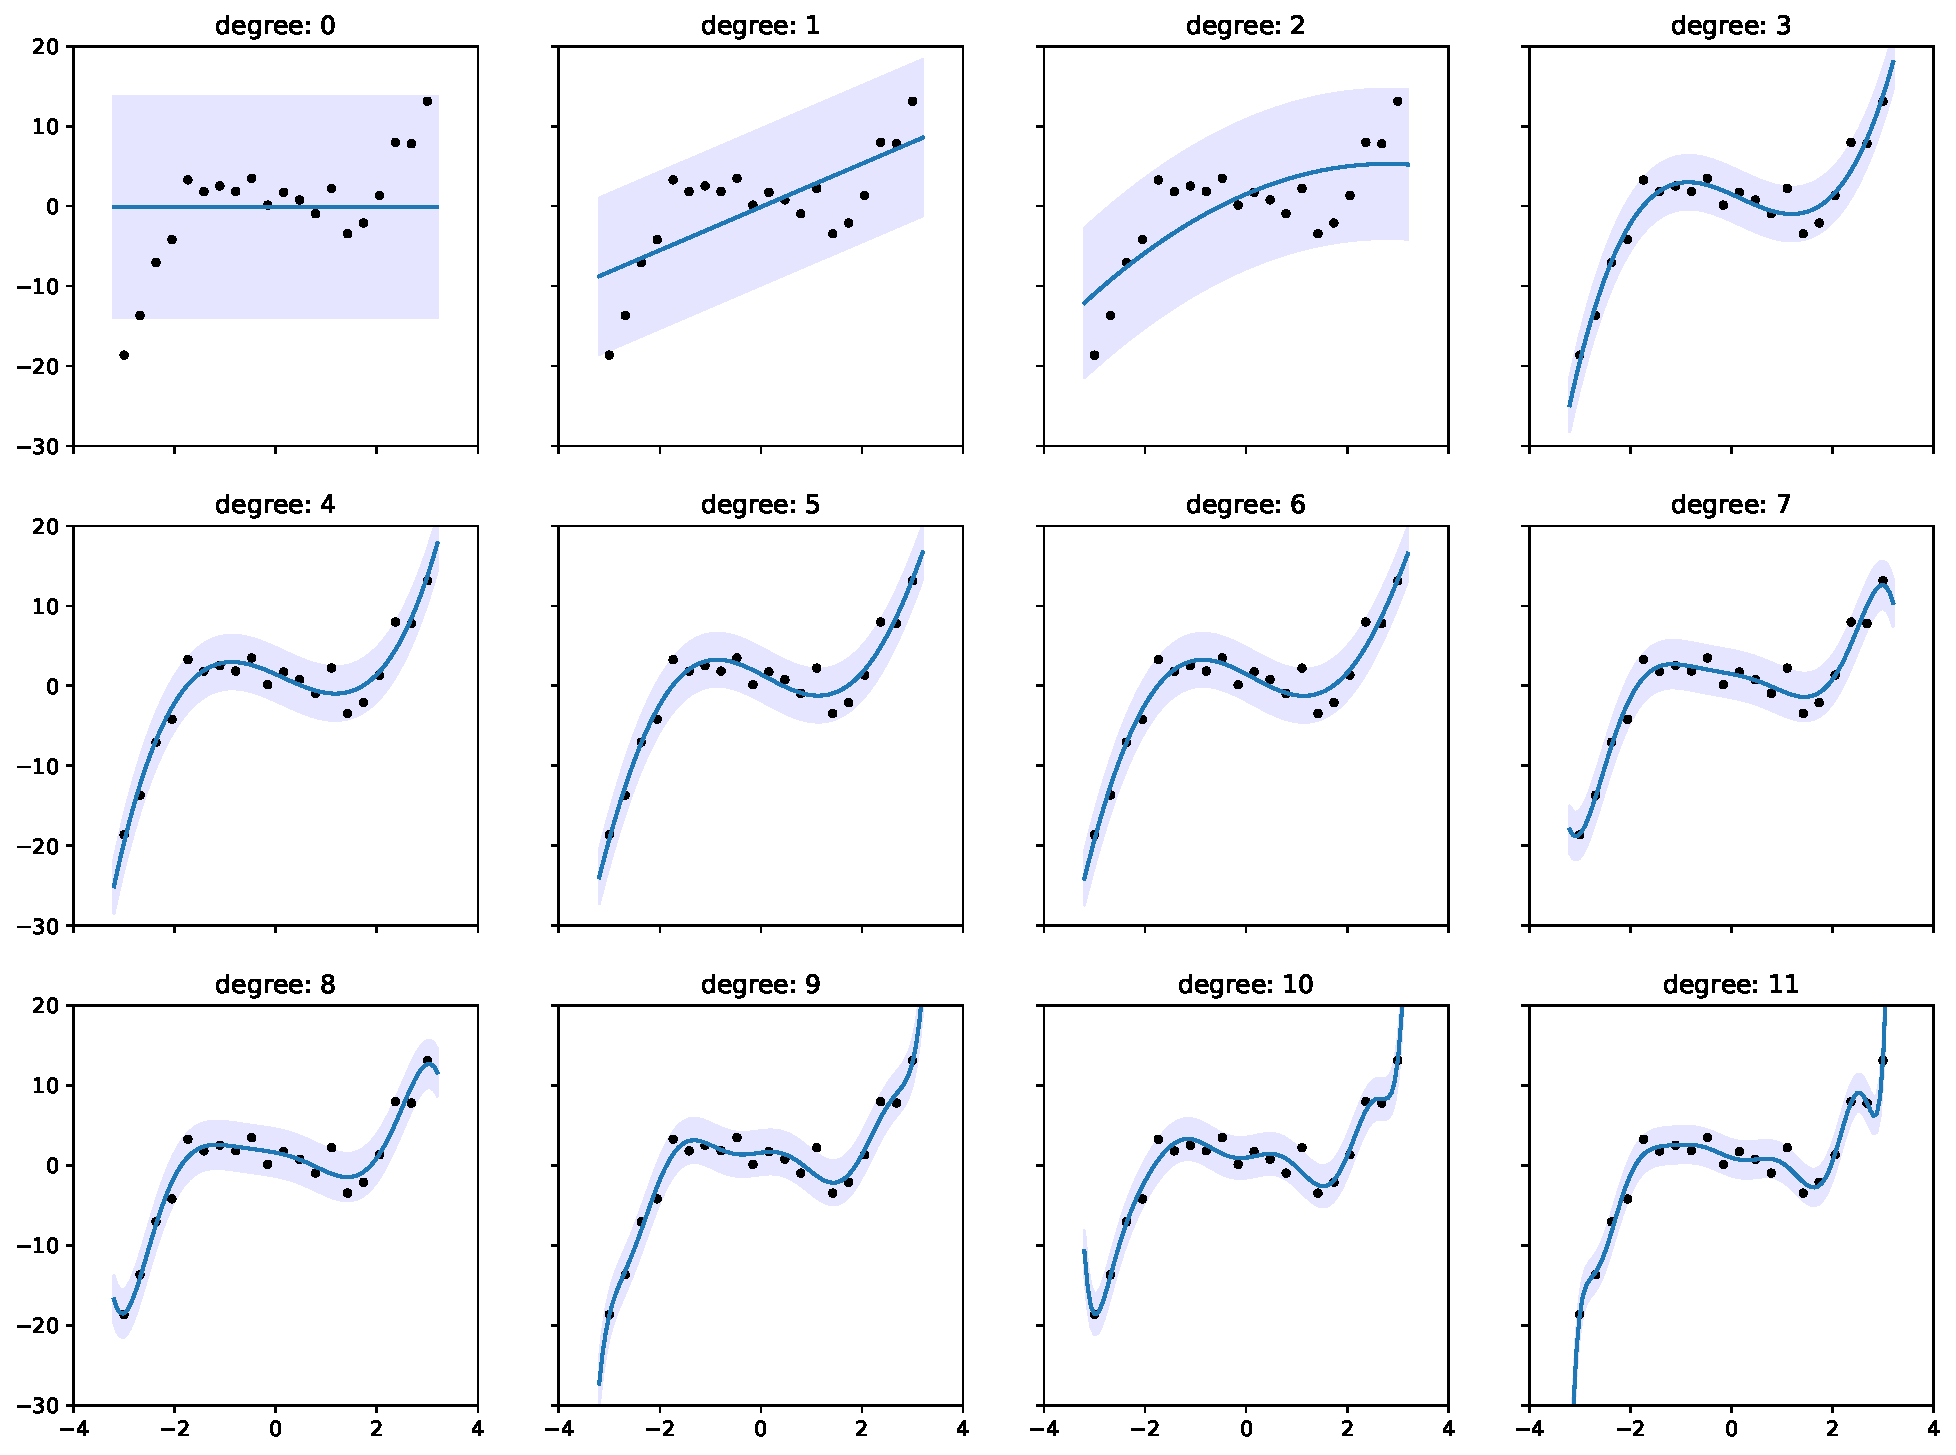
\includegraphics[width=\textwidth]{./figs/03-linear-regression-fits.pdf}
	\end{figure}

\newpage
	\item $\text{AIC}_k = -2 [L_k - (k+2)]$
\begin{lstlisting}[language=python]
def AIC(X, y, c, sigma2):
	dim = len(c) + 1
	loglike = log_likelihood(X, y, c, sigma2)
	return -2 * (loglike - dim)
\end{lstlisting}

	\item $\text{BIC}_k = -2 [L_k - \frac{\log N}{2}(k+2)]$
\begin{lstlisting}[language=python]
def BIC(X, y, c, sigma2):
	N = len(y)
	dim = len(c) + 1
	loglike = log_likelihood(X, y, c, sigma2)
	return -2 * (loglike - np.log(N)/2.0 * dim)
\end{lstlisting}

	\item $\text{LRT pvalue}_{k} = 1 - \text{cdf }\chi^2(2(L_k - L_{k-1})\;|\;\text{dof} = 1)$ \\
	(calculated against the model with one less degree)
\begin{lstlisting}[language=python]
from scipy.stats import chi2

pvalues = [np.nan]
for deg in degrees[1:]:
    L1 = loglikes[deg]
    L0 = loglikes[deg-1]
    logLR = L1 - L0
    dof = 1
    pvalue = chi2.sf(2*logLR, dof)
    pvalues.append(pvalue)
\end{lstlisting}
	\begin{figure}[h]
		\centering
		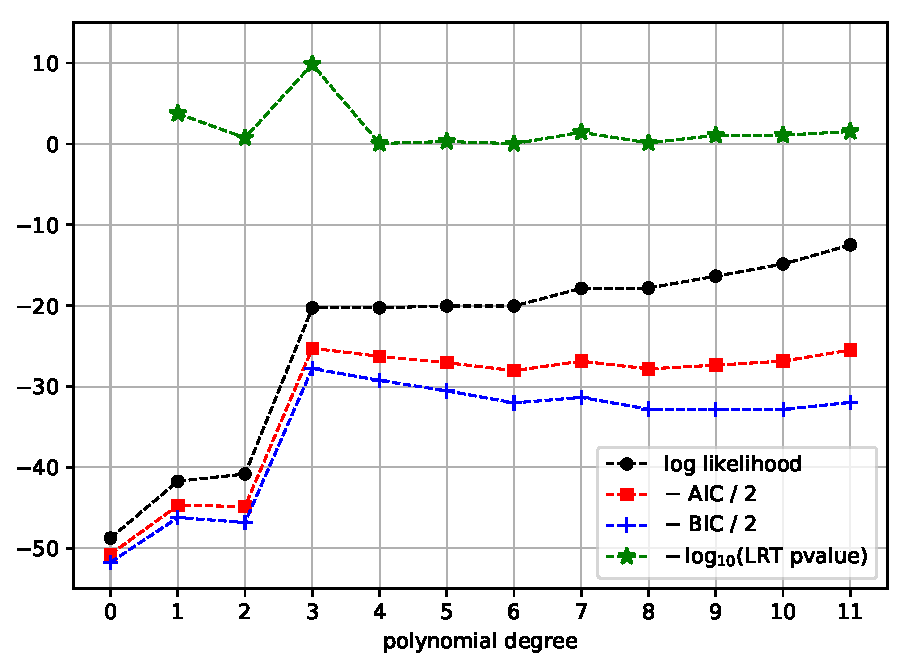
\includegraphics[width=0.75\textwidth]{./figs/03-linear-regression-LL-AIC-BIC-pvalue.pdf}
	\end{figure}

\newpage
\item BIC weights, $P(D\;|\;M_k) \approx e^{-\text{BIC}_k/2} / \sum_{k'=0}^Ke^{-\text{BIC}_{k'}/2}$
\begin{lstlisting}[language=python]
def BIC_weigths(BICs):
	BICs = np.array(BICs)
	w = BICs - np.min(BICs) # for numerical stability
	w = np.exp(-0.5*(w))  
	w /= np.sum(w)
	return w
\end{lstlisting}
	\begin{figure}[h]
		\centering
		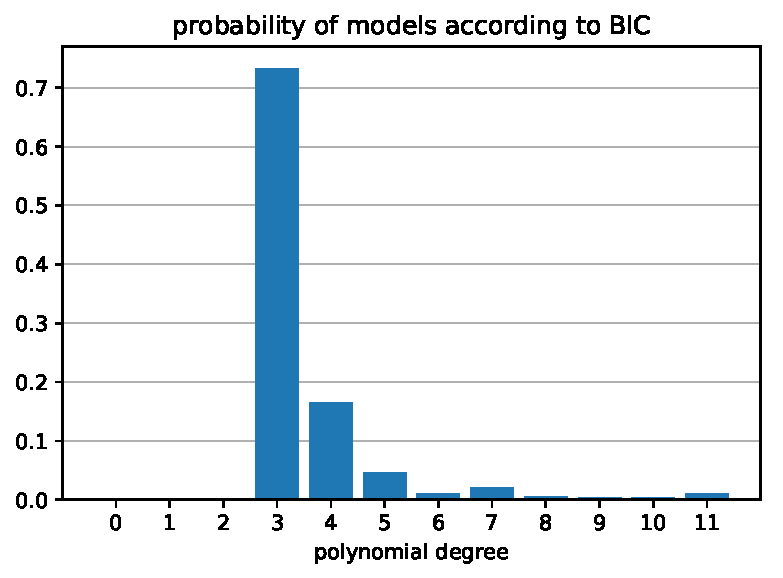
\includegraphics[width=0.7\textwidth]{./figs/03-linear-regression-BIC-weights.pdf}
	\end{figure}
\end{itemize}



\newpage
\newpage
\section{Graphical models}


\subsection{Elements}
\begin{itemize}
	\item $P(x, y) = P(y\;|\;x) P(x)$ is represented by 
	\begin{figure}[h]
	\centering
		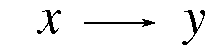
\includegraphics[height=4mm]{./figs/04-xy.pdf} 
	\end{figure}

	\item $P(x, y, z) = P(y\;|\;z,x) P(z\;|\;x) P(x)$. \\ 
	 If $P(y\;|\;z,x) = P(y\;|\;z)$, then it is represented by a {\bf chain}

	\begin{figure}[h]
	\centering
		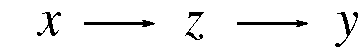
\includegraphics[height=4mm]{./figs/04-xzy.pdf} 
	\end{figure}

	Note: $y \independent x \;|\;z$, but $y \not\independent x\; | \; \emptyset$.

	\item $P(x, y_1, y_2) = P(y_1, y_2\;|\;x) P(x)$. \\
	If $P(y_1, y_2 \;|\; x) = P(y_1\;|\;x) P(y_2\;|\;x)$, then it is represented by a {\bf fork}

	\begin{figure}[h]
	\centering
		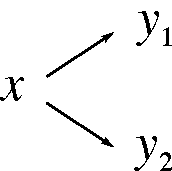
\includegraphics[height=15mm]{./figs/04-xy1y2.pdf} 
	\end{figure}

	Note: $y_1 \independent y_2 \;|\;x$, but $y_1 \not\independent y_2\; | \; \emptyset$.

	\item $P(x_1, x_2, y) = P(y\;|\;x_1, x_2) P(x_1, x_2)$. \\
	If $P(x_1, x_2) = P(x_1) P(x_2)$, then it is represented by a {\bf collider}

	\begin{figure}[h!]
	\centering
		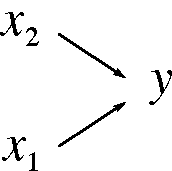
\includegraphics[height=15mm]{./figs/04-x1x2y.pdf} 
	\end{figure}

	Note: $x_1 \independent x_2\;|\;\emptyset$, but $x_1 \not\independent x_2\;|\;y$ (!).
	
\end{itemize}

\no Examples
\begin{itemize}
	\item $P(a, b, c, d, e) = P(a)P(d) P(b\;|\;a,d) P(c\;|\;b) P(e\;|\;c) P(f\;|\;c)$ is represented by 

	\begin{figure}[h!]
	\centering
		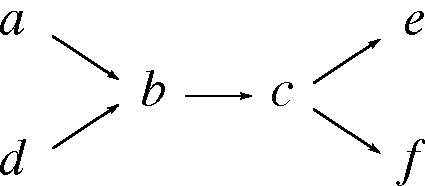
\includegraphics[height=15mm]{./figs/04-abcdef.pdf} 
	\end{figure}

	\item $P(a, b, c, d, e, f) = P(a) P(c\;|\;a) P(b\;|\;a) P(f\;|\;c) P(d\;|\;b, c) P(e\;|\;d)$ is represented by

	\begin{figure}[h!]
	\centering
		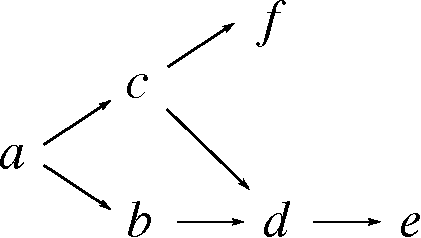
\includegraphics[height=20mm]{./figs/04-abcdef2.pdf} 
	\end{figure}
\end{itemize}

\newpage
\subsection{Real-life examples}
\begin{itemize}
	\item Fire causes Smoke, Smoke causes Alarm to set off, but given Smoke, there's no correlation between Fire and Alarm, i.e. $\text{Fire}\;\independent\;\text{Alarm}\;|\;\text{Smoke}$. This is represented by a chain
	\begin{figure}[h!]
	\centering
		
\includegraphics[height=2.8mm]{./figs/04-fire-smoke-alarm.pdf} 
	\end{figure}

	\item Both rain and the Sprinkler can cause the formation of a Puddle, they are however independent (until we observe the Puddle), i.e. $\text{Rain}\;\independent\;\text{Sprinkler}\;|\;\emptyset$. This is represented by a collider
	\begin{figure}[h!]
	\centering
		
\includegraphics[height=14mm]{./figs/04-rain-puddle-sprinkler.pdf} 
	\end{figure}

	\item Heat causes both Ice Cream sales and Crime to increase, but once we know there was a heatwave, they become independent, i.e. $\text{Crime}\;\independent\;\text{Ice Cream}\;|\;\text{Heat}$. This is represented by a fork
	\begin{figure}[h!]
	\centering
		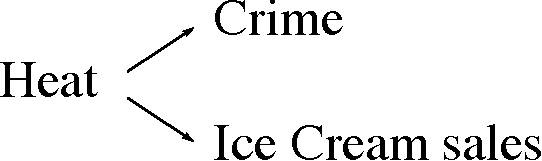
\includegraphics[height=12mm]{./figs/04-heat-icecream-crime.pdf} 
	\end{figure}

	\item Education affects Political View, which affects both Party membership and Voting behavior. This can be represented as
	\begin{figure}[h!]
	\centering
		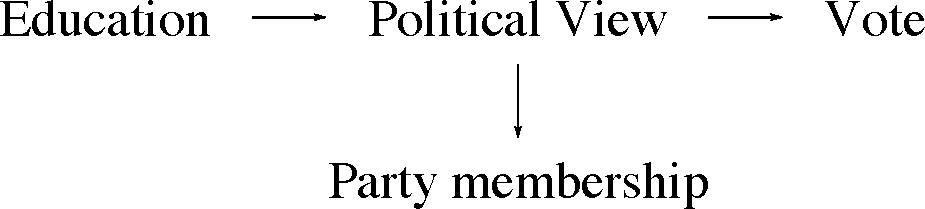
\includegraphics[height=16mm]{./figs/04-education-vote.pdf} 
	\end{figure}

	\item Education and Experience both affect Salary, but Education also affect Experience. This can be represented as
	\begin{figure}[h!]
	\centering
		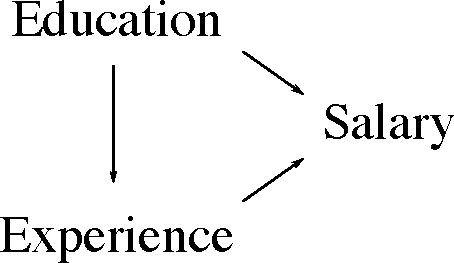
\includegraphics[height=20mm]{./figs/04-education-salary.pdf} 
	\end{figure}
\end{itemize}

\newpage
\subsection{Hierarchical models}

\no Beta-Binomial model
\begin{itemize}
	\item Data: $D = \{(k_i, n_i)\}_{i=1}^N$, where $k_i$(successes) $\in\{0, 1, \ldots n_i\}$, and $n_i$(attempts) $\in \mathds{N}$

	\item Model: 
		\begin{itemize}
			\item level 1: the parameters, $p = \{p_i\}_{i=1}^N$, where $p_i \in [0,1]$, define $P(k_i\;|\;n_i, p_i) = \text{Binomial}(k_i\;|\;n_i, p_i)$
			\item level 2: the parameters, $\alpha, \beta$ (both $>0$), define $P(p_i\;|\;\alpha, \beta) = \text{Beta}(p_i\;|\;\alpha, \beta)$.
		\end{itemize}
		This hierarchy can be represented as
		\begin{figure}[h!]
		\centering
			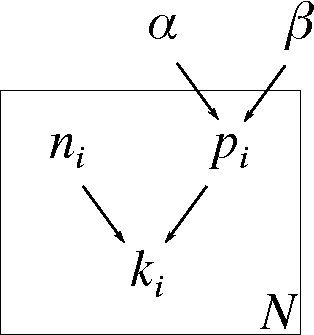
\includegraphics[height=26mm]{./figs/04-BetaBinomial.pdf}
		\end{figure}

	\item Joint likelihood:
	\be
		P(D, p\;|\;\alpha,\beta) = \prod_{i=1}^N\Big[\text{Binom}(k_i\;|\;n_i, p_i) \;\text{Beta}(p_i\;|\;\alpha, \beta)\Big]
	\ee

	\item Marginal likelihood:
	\ba
		P(D\;|\;\alpha, \beta) &=& \prod_{i=1}^N\left[\int\!dp_i\,\text{Binom}(k_i\;|\;n_i, p_i) \;\text{Beta}(p_i\;|\;\alpha, \beta)\right] = \prod_{i=1}^N\Big[\text{Beta-Binom}(k_i\;|\;n_i, \alpha, \beta)\Big]
		\\
		\text{where}&&
		\text{Beta-Binom}(k\;|\;n, \alpha, \beta) = \frac{\Gamma(n+1)\Gamma(\alpha + \beta)}{\Gamma(n + \alpha + \beta)} \frac{\Gamma(k+\alpha)}{\Gamma(k+1) \Gamma(\alpha)} \frac{\Gamma(n - k + \beta)}{\Gamma(n-k + 1) \Gamma(\beta)}
	\ea
\end{itemize}

\no Gamma-Poisson model (aka. Negative Binomial model)
\begin{itemize}
	\item Data: $D = \{k_i\}_{i=1}^N$, where $k_i$(events) $\in \mathds{N}$.
	\item Model: 
	\begin{itemize}
		\item level 1: the parameters $\lambda = \{\lambda_i\}_{i=1}^N$, where $\lambda_i$ > 0, define $P(k_i\;|\;\lambda) = \text{Poisson}(k_i\;|\;\lambda_i)$
		\item level 2: the parameters $\alpha, \beta$ (both $>0$), define $P(\lambda_i\;|\; \alpha, \beta) = \text{Gamma}(\lambda_i\;|\;\alpha, \beta)$.
	\end{itemize}
	This hierarchy can be represented as 
	\begin{figure}[h!]
		\centering
			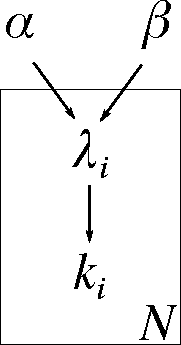
\includegraphics[height=26mm]{./figs/04-GammaPoisson.pdf}
		\end{figure}
	\item Joint likelihood:
	\be
		P(D, \lambda\;|\;\alpha, \beta) = \prod_{i=1}^N\Big[\text{Poisson}(k_i\;|\;\lambda_i) \;\text{Gamma}(\lambda_i\;|\;\alpha, \beta)\Big]
	\ee

	\item Marginal likelihood:
	\ba
		P(D\;|\;\alpha, \beta) &=& \prod_{i=1}^N\left[\int\!d\lambda_i\,\text{Poisson}(k_i\;|\;\lambda_i) \;\text{Gamma}(\lambda_i\;|\;\alpha, \beta)\right] = \prod_{i=1}^N\Big[\text{Gamma-Poisson}(k_i\;|\;\alpha, \beta)\Big]
		\\
		\text{where} && \text{Gamma-Poisson}(k\;|\;\alpha, \beta) = \frac{\Gamma(k + \alpha)}{\Gamma(k+1)\Gamma(\alpha)} \left(\frac{1}{\beta + 1}\right)^k \left(\frac{\beta}{\beta + 1}\right)^\alpha = 
		\\
		&=&
		\text{NegativeBinom}(k\;|\;r, p) = {k + r -1 \choose k} p^k (1-p)^r,\quad \text{with }r = \alpha, \; p = \frac{1}{\beta + 1}
	\ea
\end{itemize}

\no Dirichlet-Multinomial model
\begin{itemize}
	\item Data: $D = \{k_i\in\mathds{N}^M\}_{i=1}^N = \{(k_{i,1}, k_{i,2}, \ldots k_{i,M})\}_{i=1}^N$, where $k_{i,j}$(number of outcome $j$) $\in \mathds{N}$
	\item Model:
	\begin{itemize}
		\item level 1: the parameters $p = \{p_i \in \mathds{R}^{M}\}_{i=1}^N = \{(p_{i,1}, p_{i,2},\ldots p_{i,M})\}_{i=1}^N$, where $p_{i,j}$(probability of outcome $j$ in sample $i$) $>0$, and $\sum_{j=1}^M p_{i,j} = 1,\;\forall i$, define $P(k_i\;|\;p_i) = \text{Multinomial}(k_i\;|\;k_{i,\text{tot}},p_i)$, where $k_{i,\text{tot}} = \sum_{j=1}^M k_{i,j}$
		\item level 2: the parameters $\alpha = (\alpha_1, \alpha_2, \ldots \alpha_M)$, where each $\alpha_j > 0$, define $P(p_i\;|\; \alpha)= \text{Dirichlet}(p_i\;|\;\alpha)$
	\end{itemize}
	This hierarchy can be represented as 
	\begin{figure}[h!]
		\centering
			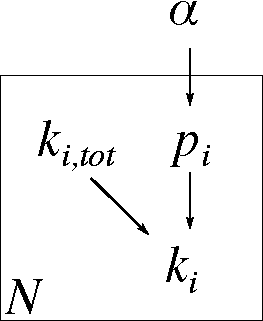
\includegraphics[height=26mm]{./figs/04-DirichletMultinomial.pdf}
		\end{figure}
	\item Joint likelihood:
	\be
		P(D\;p|\;\alpha) = \prod_{i=1}^N\Big[ \text{Multinomial}(k_i\;|\;k_{i,\text{tot}}, p_i)\;\text{Dirichlet}(p_i\;|\alpha) \Big]
	\ee
	\item Marginal likelihood:
	\ba
		P(D\;|\;\alpha) &=& \prod_{i=1}^N\left[\int\!dp_i\, \text{Multinomial}(k_i\;|\;k_{i,\text{tot}}, p_i)\;\text{Dirichlet}(p_i\;|\alpha) \right] = \prod_{i=1}^N\Big[\text{Dirichlet-Multinomial}(k_i\;|\;k_{i,\text{tot}}, \alpha)\Big]
		\\
		\text{where} && \text{Dirichlet-Multinomial}(k\;|\;k_\text{tot}, \{\alpha_j\}_{j=1}^M) = \frac{\Gamma(k_\text{tot}+1)\Gamma(\alpha_\text{tot})}{\Gamma(k_\text{tot} + \alpha_\text{tot})} \prod_{j=1}^M \frac{\Gamma(k_j + \alpha_j)}{\Gamma(k_j + 1)\Gamma(\alpha_j)},
		\\
		&&\text{where }\quad \alpha_\text{tot} = \sum_{j=1}^M \alpha_j
	\ea
\end{itemize}

\newpage
\no Bayesian ANOVA (aka. Random Effect Model)
\begin{itemize}
	\item Data: $D = \{x_g\}_{g=1}^G = \{(x_{g,1}, x_{g,2},\ldots x_{g, N_g})\}_{g=1}^G$, where $x_{g,i} \in \mathds{R}$ is measurement $i$ in group $g$, and groups can be of different sizes $N_g$.
	\item Model:
	\begin{itemize}
		\item level 1: The parameters $\mu = \{\mu_g\}_{g=1}^G$ and $\sigma^2$ define $P(x_{g,i}\;|\;\mu_g, \sigma) = \text{Normal}(x_{g,i}\;|\;\mu_g, \sigma^2)$
		\item level 2: The parameter $\sigma_0^2$ define $P(\mu_g\;|\;\mu_0,\sigma_0) = \text{Normal}(\mu_g\;|\;\mu_0, \sigma_0^2)$
	\end{itemize}
	This hierarchy can be represented as  
	\begin{figure}[h]
		\centering
			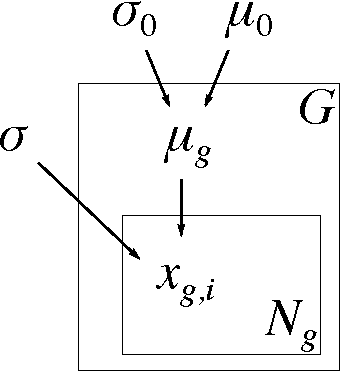
\includegraphics[height=26mm]{./figs/04-anova.pdf}
		\end{figure}
	\item Joint likelihood:
	\be
		P(D, \mu\;|\; \mu_0, \sigma_0, \sigma) = \prod_{g=1}^G\left[\text{Normal}(\mu_g\;|\;\mu_0, \sigma_0^2) \times \prod_{i=1}^{N_g}\text{Normal}(x_{g,i}\;|\;\mu_g, \sigma^2)\right]
	\ee
	\item Marginal likelihood:
	\ba
		P(D\;|\;\mu_0, \sigma_0, \sigma) 
		&=& 
		\prod_{g=1}^G\intop_{-\infty}^{+\infty}\!d\mu_g\,\left[\text{Normal}(\mu_g\;|\;\mu_0, \sigma_0^2) \times \prod_{i=1}^{N_g}\text{Normal}(x_{g,i}\;|\;\mu_g, \sigma^2)\right] 
		\\
		&=&
		(2\pi \sigma_0^2)^{-\frac{G}{2}} \prod_{g=1}^G \left[\frac{1}{\sqrt{\xi + N_g}}(2\pi\sigma^2)^{-\frac{N_g-1}{2}}\exp\left(-\frac{N_g}{2\sigma^2}\left[\frac{\xi}{\xi + N_g}(\mu_g - m_g)^2 + s_g^2\right]\right)\right]
		\\
		\text{where}&& \xi = \frac{\sigma^2}{\sigma_0^2},\qquad m_g = \frac{1}{N_g}\sum_{i=1}^{N_g} x_{g,i}, \qquad s_g^2 = \frac{1}{N_g}\sum_{i=1}^{N_g} x_{g,i}^2 - m_g^2
	\ea

\end{itemize}









\newpage
\newpage
\section{Hidden variables, EM, Mixture models}
\label{sec:EM}


\subsection{Definitions}
\begin{itemize}
	\item Known values: 
		\begin{itemize}
			\item Observations (or data), $D = \{x_i\}_{i=1}^N$
		\end{itemize}
	\item Unknown values: 
		\begin{itemize}
			\item Parameters: $\theta = \{\theta_k\}_{k=1}^K$
			\item Hidden variables (or hidden data): $Z = \{z_i\}_{i=1}^N$ (i.e. $Z$ is as numerous as $D$)
		\end{itemize}
\end{itemize}
\begin{figure}[h]
\centering
	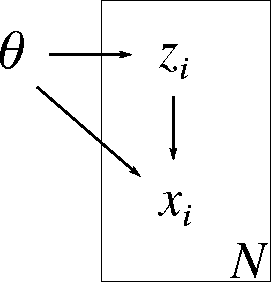
\includegraphics[height=22mm]{./figs/05-DZtheta.pdf}
\end{figure}

\subsection{Expectation Maximization}
\no Goal
\begin{itemize}
	\item Given the likelihood $P(D\;|\;Z, \theta)$, and prior on hidden variables $P(Z\;|\;\theta)$,
	\item The joint is $P(D, Z\;|\;\theta) = P(D\;|\;Z, \theta)\, P(Z\;|\;\theta)$
	\item The marginal is $P(D\;|\;\theta) = \sum_Z P(D, Z\;|\;\theta)$
	\item We wish to find $\theta$ that maximizes the marginal, i.e.
	\be
		\theta^\text{MLE} = \amax_{\theta} \Big[\log P(D \;|\; \theta)\Big] = \amax_{\theta} \left[\log \Big(\sum_Z P(D, Z\;|\;\theta)\Big)\right]
	\ee
	\item Direct numerical optimization is usually feasible, but the EM method is often faster.
\end{itemize}


\no Expectation Maximization (EM) algorithm:
\begin{enumerate}
	\item Start with realistic $\theta = \theta^\text{old}$
	\item E-step: Calculate $P(Z\;|\;D,\theta^\text{old}) = \frac{P(D, Z\;|\;\theta^\text{old})}{\sum_{Z'} P(D,Z'\;|\;\theta^\text{old})}$
	\item M-step: Find the optimal $\theta = \theta^\text{new}$ that maximizes $\sum_Z P(Z\;|\;D,\theta^\text{old})\log P(D,Z\;|\;\theta)$
	\item Set $\theta^\text{old} \leftarrow \theta^\text{new}$, check convergence, and return to E-step if needed.
\end{enumerate}

\begin{itemize}
	\item The one-liner iteration formula is based on the joint $P(D,Z\;|\;\theta)$:
	\be
		\theta^\text{new} = \amax_\theta\left[\sum_Z \frac{P(D, Z\;|\; \theta^\text{old})}{\sum_{Z'} P(D, Z'\;|\; \theta^\text{old})} \log P(D, Z\;|\; \theta)\right]
	\ee
\end{itemize}


\newpage
\subsection{Mixture models}
\begin{itemize}
	\item Data: $D=\{x_i\}_{i=1}^N$
	\item Parameters: $\theta, w$ 
		\begin{itemize}
			\item Components: $c \in \{1, 2, \ldots C\}$
			\item Parameters for each component $\theta = \{\theta_c\}_{c=1}^C$
			\item Mixing proportions: $w = \{w_c \in [0,1]\}_{c=1}^C$, such that $\sum_c w_c = 1$.
		\end{itemize}
	\item Hidden variables: labels $L = \{l_i\}_{i=1}^N$, where $l_i\in \{1, 2, \ldots C\}$
	\item Model: mixture of distinct distributions
		\begin{itemize}
			\item Generative distribution for each component: $P(x_i\;|\;l_i = c, \theta) = P(x_i\;|\;\theta_c)$
			\item Probability of an observation coming from a component: $P(l_i = c) = w_c$
		\end{itemize}
	
	\begin{figure}[h]
	\centering
		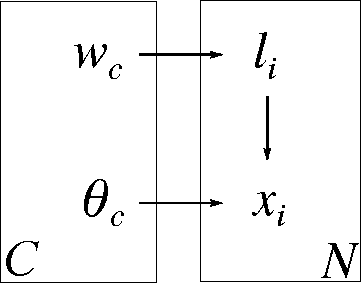
\includegraphics[height=22mm]{./figs/05-mixture.pdf}
	\end{figure}
	\item Joint
	\be
		P(D, L\;|\; \theta, w) = P(D\;|\;L, \theta) \;P(L\;|\;w) = \prod_{i=1}^N P(x_i\;|\;\theta_{l_i})\; w_{l_i}
	\ee
	\item Marginal
	\be
		P(D\;|\; \theta, w) = \sum_L P(D, L\;|\; \theta, w) = \prod_{i=1}^N\left[\sum_{c=1}^C w_c\, P(x_i\;|\;\theta_c) \right]
	\ee
\end{itemize}

\no EM algorithm
\begin{enumerate}
	\item Start with initial values: $\theta^\text{old}, w^\text{old}$
	\item In E-step, calculate
	\be	
		P(l_i = c\;|\;x_i,\theta^\text{old}) = \frac{w^\text{old}_c P(x_i\;|\;\theta^\text{old}_c)}{\sum_{c'} w^\text{old}_{c'} P(x_i\;|\;\theta^\text{old}_{c'})} =: r_{i,c}
	\ee
	\item In M-step, calculate
	\ba
		w_c^\text{new} &=& \frac{1}{N} \sum_{i=1}^N r_{i,c} 
		\\
		\theta_c^\text{new} &=& \amax_{\theta_c} \left[\sum_{i=1}^N r_{i,c} \log P(x_i\;|\;\theta_c)\right] 
		\\
		&=& \text{MLE of $\theta$ with data weights }\{r_{i,c}\}_{i=1}^N
	\ea
\end{enumerate}

\newpage
\subsection{Gaussian Mixture Model}
\no (aka. GMM or ``soft K-means clustering'')
\begin{itemize}
	\item Data: $\{x_i\}_{i=1}^N$, where $x_i \in \mathds{R}^d$ (point in $d$ dimension)
	\item Parameters:
	\begin{itemize}
		\item Clusters: $k \in \{1, 2, \ldots K\}$
		\item Mixture proportions: $\{w_k \in [0,1]\}_{k=1}^K$, where $\sum_k w_k = 1$
		\item Cluster means: $\mu = \{\mu_k \in \mathds{R}^d\}_{k=1}^K$
		\item Cluster covariances: $\Sigma = \{\Sigma_k \in \mathds{R}^{d\times d}, \text{positive definite}\}_{k=1}^K$.
	\end{itemize}
	\item Hidden variables: cluster labels, $L = \{l_i\}_{i=1}^N$, where $l_i \in \{1, 2,\ldots K\}$
	\item Model
	\ba
		P(l_i = k) &=& w_k
		\\
		P(x_i\;|\;l_i=k, \mu, \Sigma) &=& \text{Normal}(x_i\;|\;\mu_k, \Sigma_k) = \frac{1}{\sqrt{\det (2\pi \Sigma_k)}} \exp\left(-\frac{1}{2}(x_i - \mu_k)^\top (\Sigma_k)^{-1}(x_i - \mu_k)\right)
	\ea
	\item Marginal:
	\be
		P(D\;|\;\mu, \Sigma, w) = \prod_{i=1}^N\left[\sum_{k=1}^K w_k\, \text{Normal}(x_i\;|\;\mu_k, \Sigma_k)\right]
	\ee
	\item EM algorithm
	\begin{enumerate}
		\item Choose realistic $w^\text{old}, \mu^\text{old}, \Sigma^\text{old}$ initial values.
		\item In E-step, calculate
		\be
			r_{i,k} = \frac{w^\text{old}_k \,\text{Normal}(x_i\;|\;\mu^\text{old}_k,\Sigma^\text{old}_k)}{\sum_{k'} w^\text{old}_{k'} \,\text{Normal}(x_i\;|\;\mu^\text{old}_{k'},\Sigma^\text{old}_{k'})}
		\ee
		\item In M-step, calculate
		\ba
			w_k^\text{new} &=& \frac{1}{N} \sum_{i=1}^N r_{i,k} 
			\\
			\mu_k^\text{new} &=& \frac{1}{w_k^\text{new} N } \sum_{i=1}^N r_{i,k} \,x_i \\
			\Sigma_k^\text{new} &=& \frac{1}{w_k^\text{new} N } \sum_{i=1}^N r_{i,k} (x_i - \mu_k^\text{new}) (x_i - \mu_k^\text{new})^\top
		\ea
	\end{enumerate}
\end{itemize}

\newpage
\no The following python class implements the EM algorithm for fitting GMM.
\begin{lstlisting}[language=python]
class GmmEm:
    def __init__(self, x):
        self.x = np.array(x)
        self.N, self.d = self.x.shape
        self.K = None
        self.weights = None
        self.means = None
        self.covs = None
    
    def initialize(self, K):
        self.K = K
        m0 = np.mean(x, axis=0)
        cov0 = np.cov(x.T)

        self.weights = [1.0/K] * K
        self.means = multivariate_normal.rvs(mean=m0, cov=cov0, size=K)
        cov_values, _ = np.linalg.eig(cov0)
        self.covs = np.array([np.eye(self.d) * 0.1 *cov_values.max()
                             for _ in range(K)])
        
    def e_step(self):
        r = []
        for k in range(K):
            r.append(self.weights[k] * 
                     multivariate_normal.pdf(self.x, 
                                             mean=self.means[k],
                                             cov=self.covs[k]))
        r = np.array(r).T
        r_sum = np.einsum('ik->i', r)
        r = np.einsum('ik,i->ik', r, 1.0/r_sum)
        return r
    
    def m_step(self, r):
        weights_new = 1.0/N * np.einsum('ik->k', r)
        means_new = 1.0/N * \
                    np.einsum('k, ik,id->kd', 
                              1.0/weights_new, 
                              r, 
                              self.x)
        deviations = np.array([self.x - means_new[k] for k in range(self.K)])
        covs_new = 1.0/N * \
                    np.einsum('k,ik,kid,kiD->kdD', 
                              1.0/weights_new, 
                              r, 
                              deviations, 
                              deviations)
        
        self.weights = weights_new
        self.means = means_new
        self.covs = covs_new
\end{lstlisting}

\newpage
\no Example: GMM in 2D with $K=2$
\begin{figure}[h]
\centering
	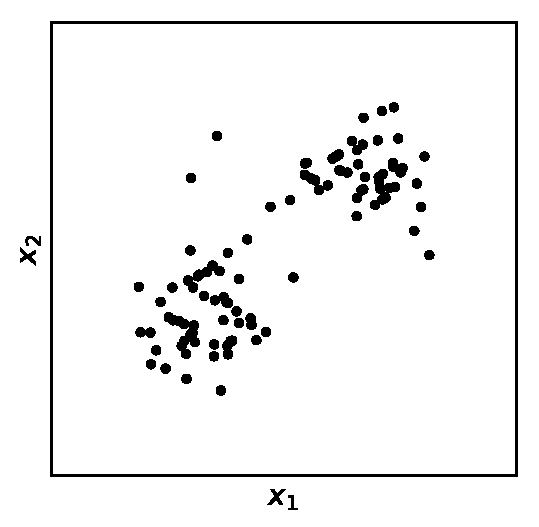
\includegraphics[width=0.30\textwidth]{./figs/05-gmm-data.pdf}
\end{figure}

\no Iterating the E- and M-steps a couple of times, we arrive to the final set of $r$ values.
\begin{lstlisting}[language=python]
gmm = GmmEm(x)

K = 2
gmm.initialize(K)
for it in range(12):
    r = gmm.e_step()
    gmm.m_step(r)
\end{lstlisting}

\begin{figure}[h!]
\centering
	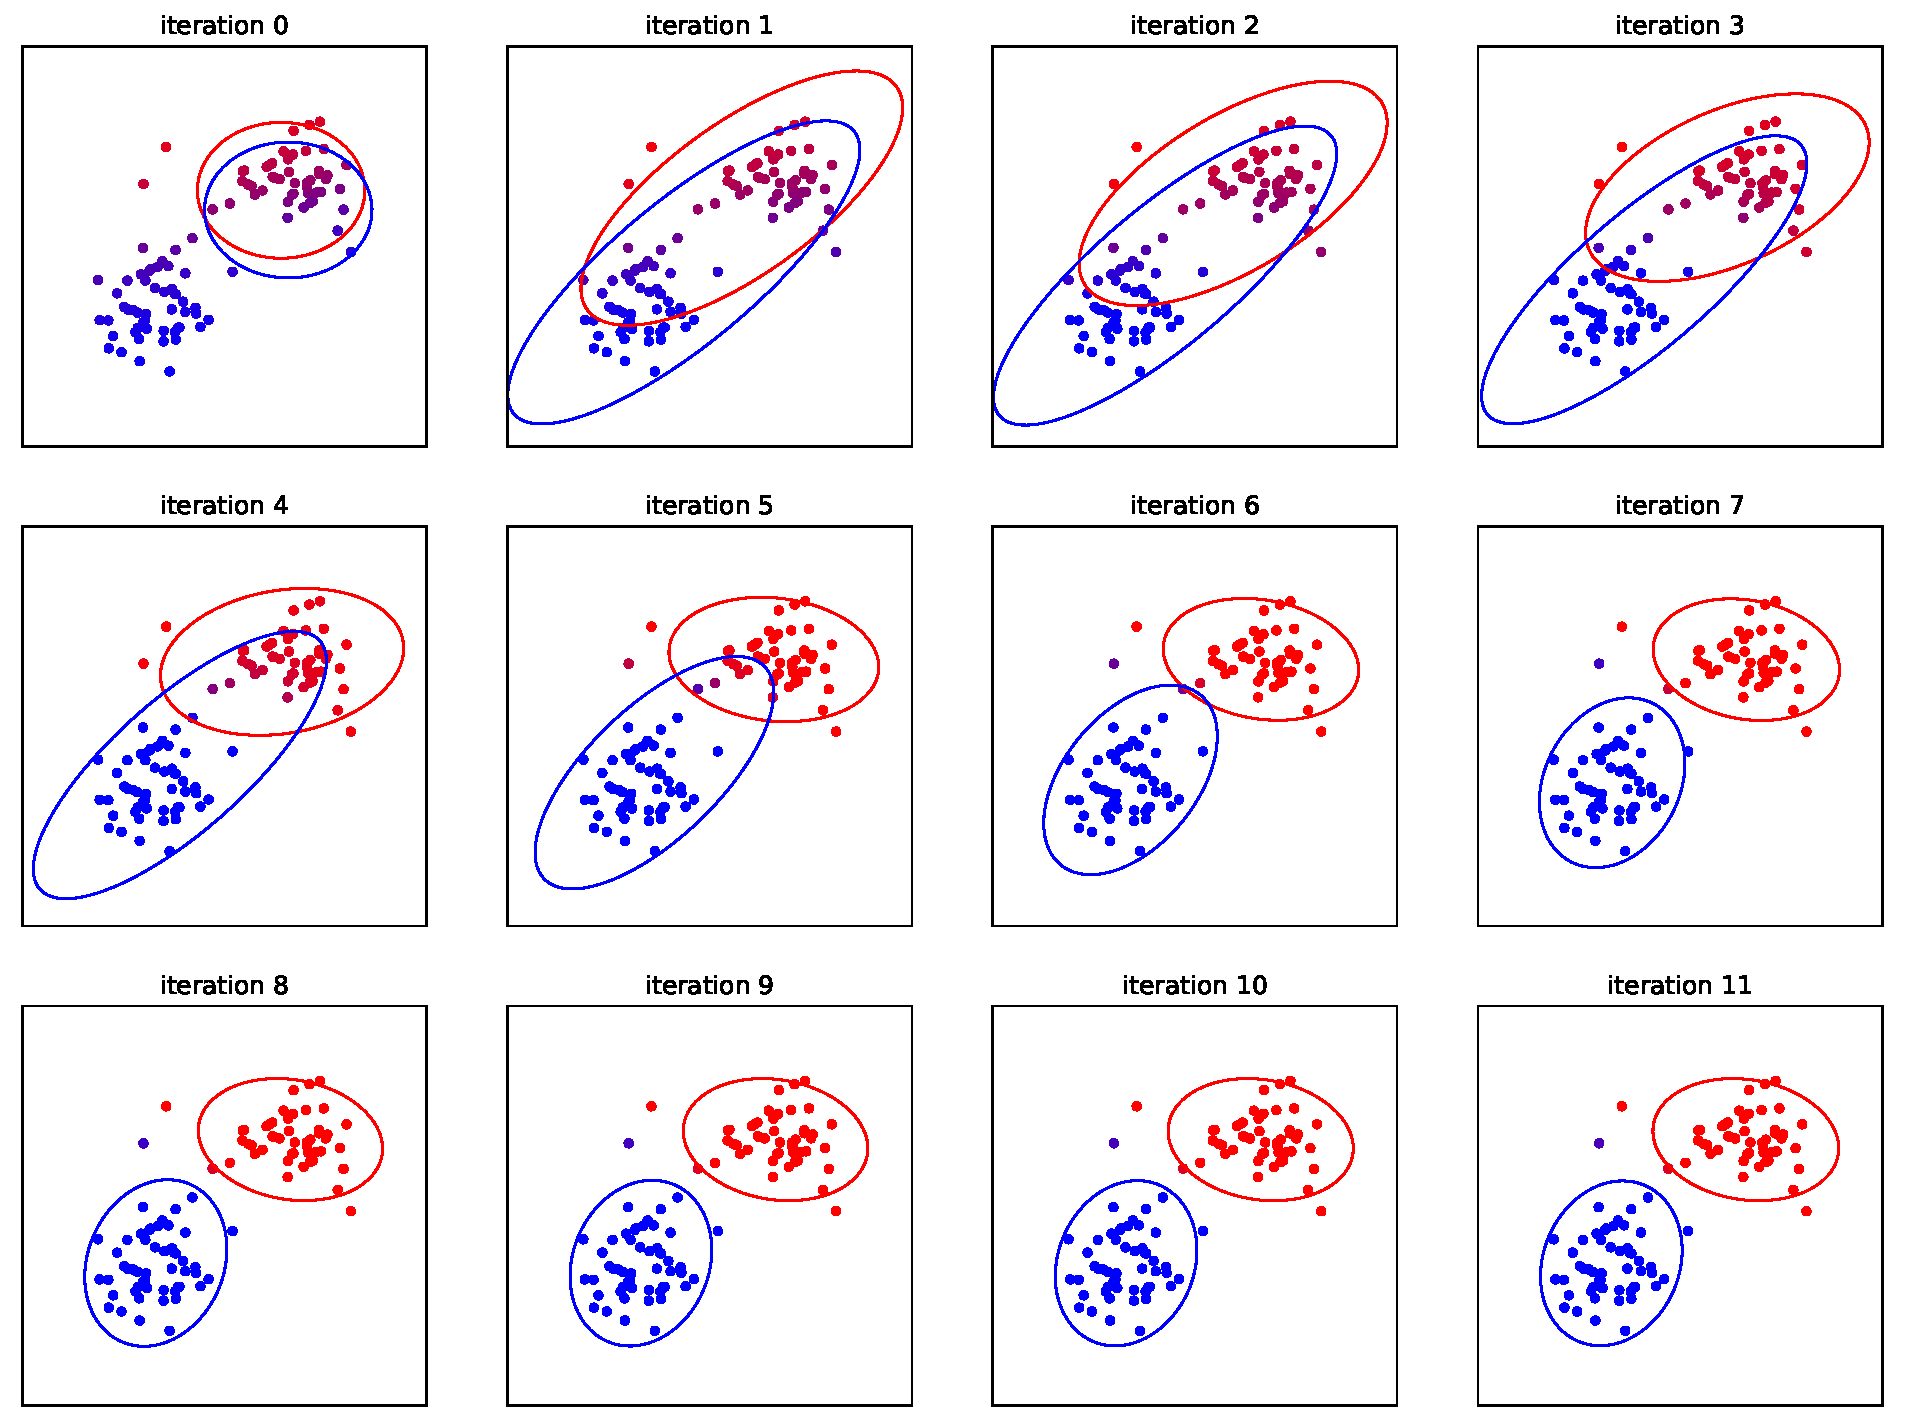
\includegraphics[width=0.93\textwidth]{./figs/05-gmm-iterations.pdf}
\end{figure}







\newpage
\section{Curse of Dimensionality, Laplace approximation}


\subsection{High-dimensional example}
\begin{itemize}
	\item Data: $D = \{k_t\}_{t=1}^T$, where $k_t\in\mathds{N}$ is the number of influenza cases at small clinic on each day of the year ($T = 365$).
	\item Parameters: 
	\begin{itemize}
		\item $\theta = \{\theta_t\}_{t=1}^T$, with $\theta_t = \log(\lambda_t)$ where $\lambda_t > 0$ is the intensity of influenza on a given day $t$.
		\item $\sigma > 0$, the typical change $\theta_t - \theta_{t-1}$. 
	\end{itemize}
	\item Model:
	\begin{itemize}
		\item Prior: $P(\theta_t\;|\;\theta_{t-1}) = \text{Normal}(\theta_t\;|\;\theta_{t-1}, \,\sigma^2)$, and $P(\sigma) = \text{const.}$
		\item Data generation process: $P(k_t\;|\;\theta_t) = \text{Poisson}(k_t\;|\; \lambda = \exp(\theta_t))$
	\end{itemize}
	\item Posterior: 
	\be
		P(\theta\;|\;D) = \frac{1}{Z} P\s(\theta\;|\;D) = \frac{1}{Z} \prod_{t=1}^T \Big[ P(\theta_{t}\;|\;\theta_{t-1}) \,P (k_t\;|\;\theta_t) \Big]
	\ee
	with the understanding that $``P(\theta_1\;|\;\theta_0)'' = 1$.
	Here $Z$ is the normalization constant.
	\begin{figure}[h]
	\centering
		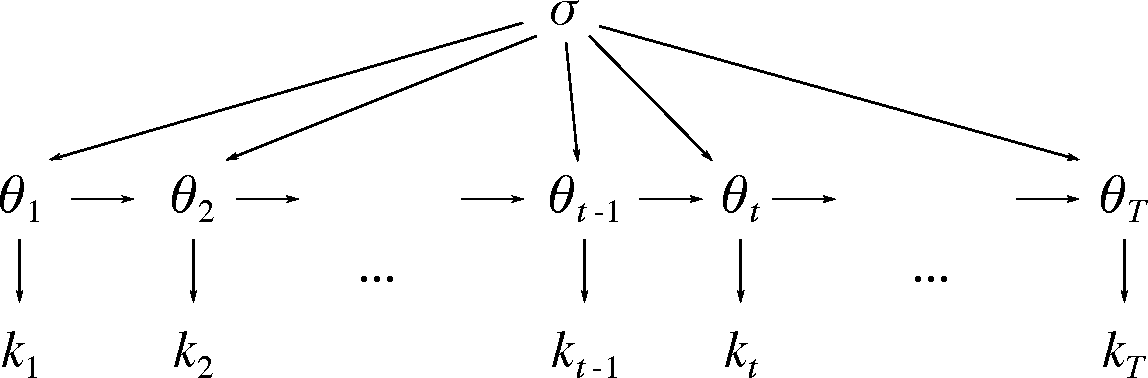
\includegraphics[width=0.5\textwidth]{./figs/06-influenza.pdf}
	\end{figure}
	\item Numerical solution would require evaluating $P\s$ on a grid of different $\theta$ values. Even, at the very extreme, when we consider only 2 values for each $\theta_t$, the number of evaluations becomes
	\be
		2^{365} \approx 10^{109} > 10^{86} \text{ (the number of protons in the observable part of the universe),}
	\ee
	which makes it impossible to pursue this strategy.
\end{itemize}

\subsection{Laplace approximation}
\begin{itemize}
	\item Goal: Determine posterior mean and variance of each parameter $\theta_t$
	\item Challenge: The dimension of $\theta = \{\theta_t\}_{t=1}^T$, i.e. $T$ is too high for direct numerical evaluation.
	\item Method: Approximate $P\s(\theta\;|\;D)$ near its maximum with a multi-variate normal distribution.
	\ba
		P\s(\theta\;|\;D) 
		&\approx& 
		\text{Normal}(\theta\;|\;\mu, \Sigma) = \frac{1}{\sqrt{\det(2\pi \Sigma)}} \exp\left[-\frac{1}{2}(\theta - \mu)^\top \Sigma^{-1} (\theta - \mu)\right]
		\\
		\\
		\text{where} 
		&&
		\mu = \amax_\theta \big[\log P\s\big] \qquad \in \mathds{R}^T
		\\
		&& \Sigma = \left[-\frac{d}{d\theta}\frac{d}{d\theta} \log P\s\right]^{-1}_{\theta = \mu} \hspace{1.9mm} \in \mathds{R}^{T\times T}
	\ea
	where $\mu$ can be found with direct numerical or analytical minimization or an expectation maximization algorithm, and $\Sigma$ can be evaluated analytically or approximated numerically.
\end{itemize}

\newpage
\subsection{Example: $(x,y)$ linear regression}
\begin{itemize}
	\item Data: $D = \{D_x, D_y\}$, 
	\begin{itemize}
		\item where $D_x = \{x_i\}_{i=1}^N = [21, 24, 17, 39, 23, 45, 33, 26, 13, 35]$, 
		\item and $\quad D_y = \{y_i\}_{i=1}^N = [22, 27, 22, 29, 26, 36, 30, 26, 15, 37]$
	\end{itemize}
	\begin{figure}[h]
	\centering
		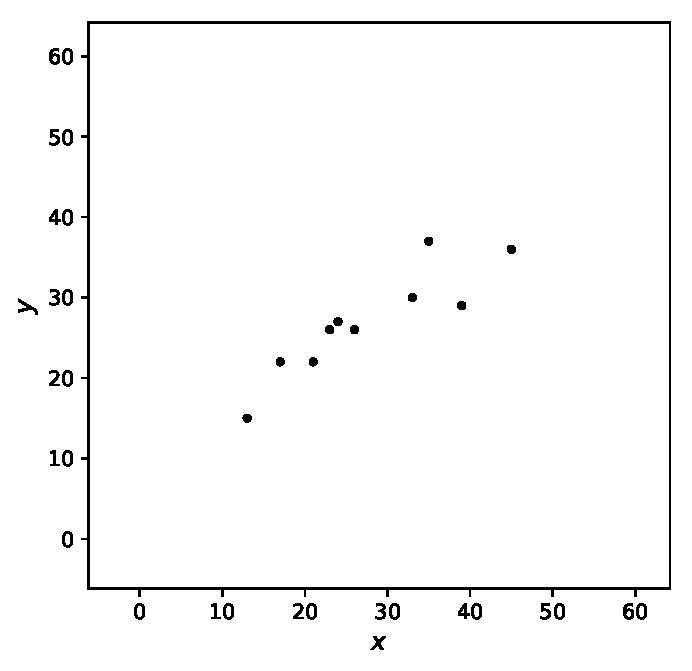
\includegraphics[width=0.38\textwidth]{./figs/06-data.pdf}
\end{figure}
	\item Parameters: $a$ (slope), $b$ (intercept), $\sigma^2$ (strength of $y$-noise), using flat priors, i.e. $P(a, b, \sigma^2) = \text{const.}$
	\item Model:
		\be
			P(D_y\;|\;D_x, a, b, \sigma^2) = \prod_{i=1}^N \text{Normal}(y_i\;|\;\mu(x_i), \sigma^2),\qquad \text{where } \mu(x_i) = ax_i + b
		\ee
	\item Unnormalized posterior:
		\be
			\log P\s(a, b, \sigma^2\;|\;D) = -\frac{N}{2}\log(2\pi \sigma^2) - \frac{1}{2\sigma^2}\sum_{i=1}^N\Big[y_i - (ax_i + b)\Big]^2
		\ee
	\item MLE estimate:
		\be
			\left.
				\begin{array}{l}
				0 = \frac{\partial}{\partial a} \log P\s = \frac{1}{\sigma^2}\left[\sum_i y_i x_i - a \sum_i x_i^2 - b \sum_i x_i\right]
				\\
				0 = \frac{\partial}{\partial b} \log P\s = \frac{1}{\sigma^2}\left[\sum_i y_i - a\sum_i x_i - bN\right]
				\\
				0 = \frac{\partial}{\partial (\sigma^2)} \log P\s = -\frac{N}{2\sigma^2} + \frac{1}{2(\sigma^2)^2} \sum_i\Big[y_i - (ax_i + b)\Big]^2
				\end{array}
			\right\}
			\Rightarrow
			\left\{
				\begin{array}{l}
				a_\text{MLE} = \big(\overline{yx} - \overline{y}\,\overline{x}\big) / \big(\overline{x^2} - \overline{x}^2\big)
				\\
				b_\text{MLE} = \overline{y} - a_\text{MLE}\,\overline{x}
				\\
				(\sigma^2)_\text{MLE} = \frac{1}{N}\sum_i\big[y_i - (a_\text{MLE}\,x_i + b_\text{MLE})\big]^2
				\end{array}
			\right.
		\ee
		where
		\be
			\overline{x} = \frac{1}{N}\sum_i x_i = 27.6,\qquad 
			\overline{y} = \frac{1}{N}\sum_i y_i = 27.0,\qquad
			\overline{x^2} = \frac{1}{N}\sum_i x_i^2 = 854.0,\qquad
			\overline{yx} = \frac{1}{N}\sum_i y_i x_i = 798.9,\qquad
		\ee
\begin{lstlisting}[language=python]
import numpy as np

def xy_linear_regression_MLE(x, y):
    N = len(x)
    ev_x = np.mean(x)
    ev_y = np.mean(y)
    ev_xx = np.mean(x * x)
    ev_yx = np.mean(y * x)
    ev_yy = np.mean(y * y)

    a_MLE = (ev_yx - ev_y * ev_x) / (ev_xx - ev_x**2)
    b_MLE = ev_y - a_MLE * ev_x
    sigma2_MLE = 1.0/N * np.sum((y - (a_MLE * x + b_MLE))**2)
    
    return a_MLE, b_MLE, sigma2_MLE
\end{lstlisting}
		giving $\mu = (a_\text{MLE}, b_\text{MLE}, (\sigma^2)_\text{MLE})$, with $a_\text{MLE} = 0.5822$, \quad $b_\text{MLE} = 10.93$, \quad  $(\sigma^2)_\text{MLE} = 7.737$.

	\item Laplace approximation:\\
	First, we calculate all second order derivatives at the MLE point:
	\ba
		\frac{\partial}{\partial a}\frac{\partial}{\partial a} \log P\s &=& -\frac{N}{\sigma^2} \overline{x^2}
		\\
		\frac{\partial}{\partial b}\frac{\partial}{\partial a} \log P\s = \frac{\partial}{\partial a}\frac{\partial}{\partial b} \log P\s &=& -\frac{N}{\sigma^2}\overline{x}
		\\
		\frac{\partial}{\partial b}\frac{\partial}{\partial b} \log P\s &=& -\frac{N}{\sigma^2}
		\\
		\frac{\partial}{\partial (\sigma^2)}\frac{\partial}{\partial a} \log P\s = \frac{\partial}{\partial a}\frac{\partial}{\partial (\sigma^2)} \log P\s &=& 0
		\\
		\frac{\partial}{\partial (\sigma^2)}\frac{\partial}{\partial b} \log P\s = \frac{\partial}{\partial b}\frac{\partial}{\partial (\sigma^2)} \log P\s &=& 0 
		\\
		\frac{\partial}{\partial (\sigma^2)} \frac{\partial}{\partial (\sigma^2)} \log P\s &=& -\frac{N}{2(\sigma^2)^2}
	\ea
	from which we construct the second derivative at the MLE point:
	\be
		\left.-\nabla\nabla \log P\s\right|_\text{MLE} = 
		\frac{N}{(\sigma^2)_\text{MLE}}
		\threebythreematrix
		{\overline{x^2}}{\overline{x}}{0}
		{\overline{x}}{1}{0}
		{0}{0}{\frac{1}{2(\sigma^2)_\text{MLE}}}
	\ee
\begin{lstlisting}[language=python]
minus_dd_logPstar = N / sigma2_MLE * \
np.array([
    [ev_xx, ev_x, 0],
    [ev_x, 1, 0],
    [0, 0, 1/(2*sigma2_MLE)]
])
Sigma = - np.linalg.inv(minus_dd_logPstar)
\end{lstlisting}
	giving 
	\be
		\Sigma = \Big[-\nabla\nabla \log P\s|_\text{MLE}\Big]^{-1} = \threebythreematrix
		{0.0839}{-0.2315}{0.0}
		{-0.2315}{7.1634}{0.0}
		{0.0}{0.0}{11.197}
	\ee
	and
	\ba
		\text{Var}(a\;|\;D) &\approx& \Sigma_{1,1} = 0.0839,\\
		\text{Var}(b\;|\;D) &\approx& \Sigma_{2,2} = 7.1634,\\
		\text{Var}(\sigma^2\;|\;D) &\approx& \Sigma_{3,3} = 11.197
	\ea
\end{itemize}
\begin{figure}[h]
	\centering
		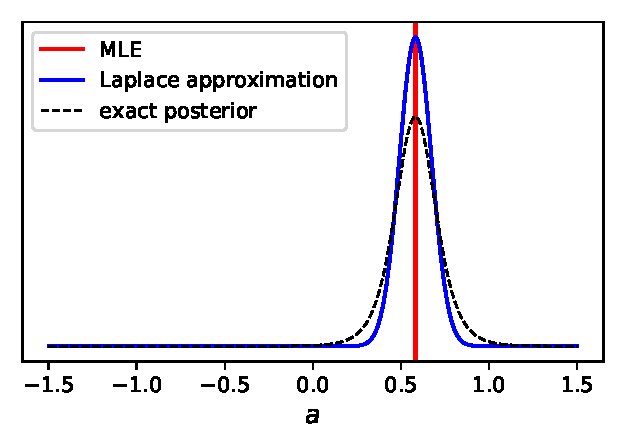
\includegraphics[width=0.45\textwidth]{./figs/06-a.pdf}
		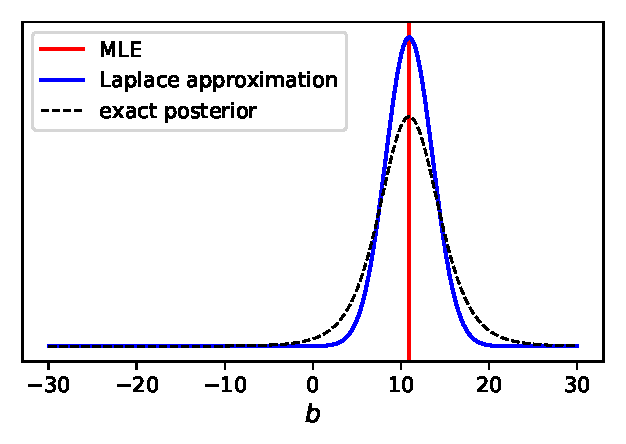
\includegraphics[width=0.45\textwidth]{./figs/06-b.pdf}\\
		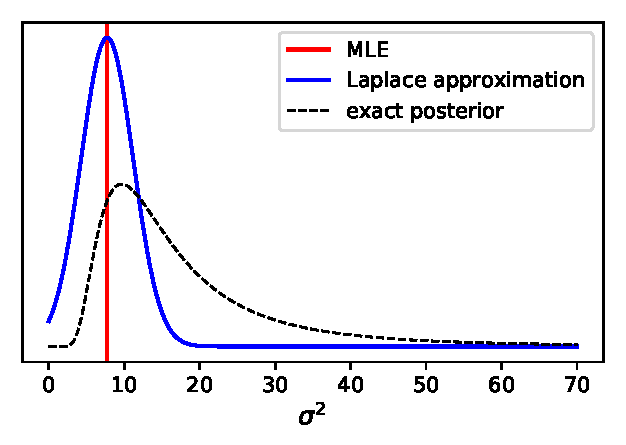
\includegraphics[width=0.45\textwidth]{./figs/06-sigma2.pdf}
\end{figure}
\begin{figure}[h]
	\centering
		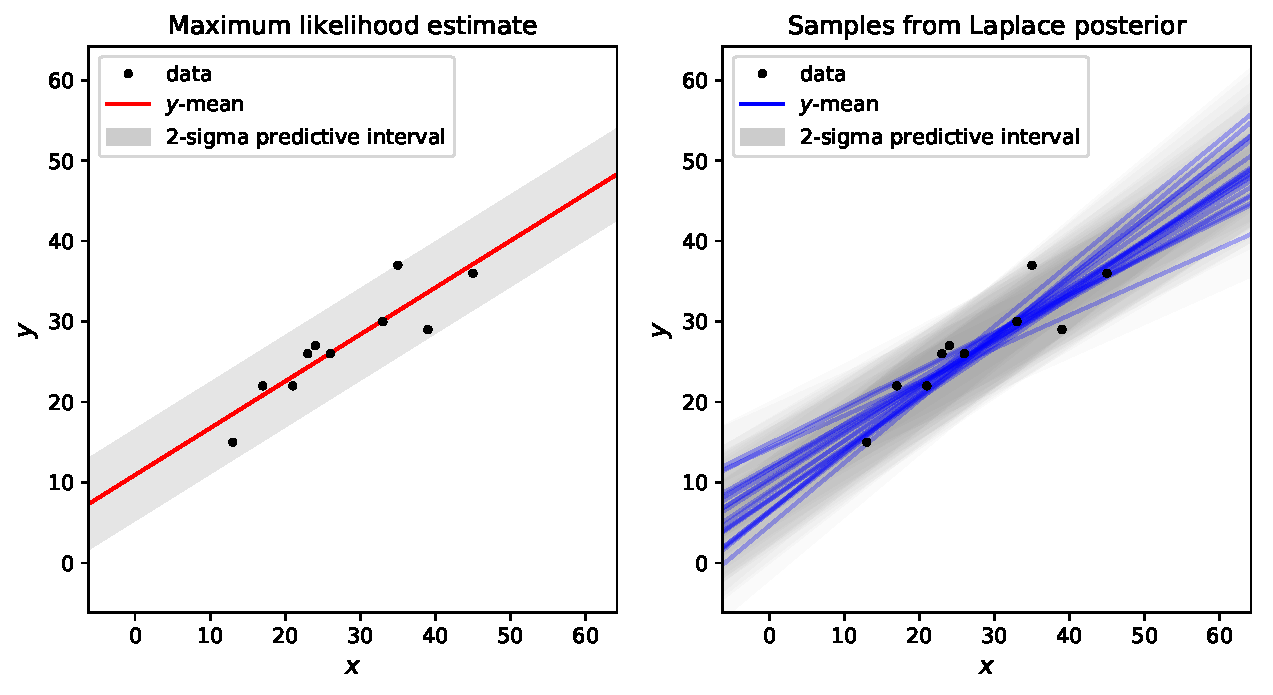
\includegraphics[width=\textwidth]{./figs/06-linear-regression.pdf}
\end{figure}













\newpage
\clearpage
\section{Monte Carlo methods}

\subsection{Monte Carlo simulation}
\begin{itemize}
	\item {\bf Goal:} Analyze complicated distributions by drawing samples from them: $P(\theta) \mapsto \{\theta^{(s)}\}$. 
	\item {\bf Challenge:} From the vast majority of distributions, we don't know how to draw samples efficiently.
	\item {\bf Method:} 
	\begin{enumerate}
		\item Draw samples from an easy-to-sample distribution.
		\item Transform the drawn values so they become samples from the distribution of question.
	\end{enumerate}
\end{itemize}
\begin{figure}[h]
\centering
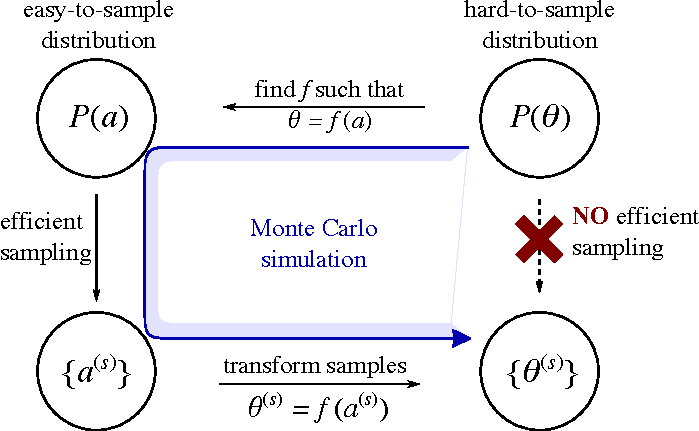
\includegraphics[width=0.5\textwidth]{./figs/07-MC.pdf}
\end{figure}


\no {\bf Example:} Ratio of two normal variables
\begin{itemize}
	\item Input: $P(x_1) = \text{Normal}(x_1\;|\;0, 1)$, $P(x_2) = \text{Normal}(x_2\;|\;0, 1)$
	\item Output: $y := x_1 / x_2$, $P(y) = \;?$
	\item MC method:
\begin{lstlisting}[language=python]
from scipy.stats import norm

samples = 1000
X1 = norm.rvs(loc=0, scale=1, size=samples)
X2 = norm.rvs(loc=0, scale=1, size=samples)
Y = X1 / X2
\end{lstlisting}

\end{itemize}

\begin{figure}[h]
\centering
	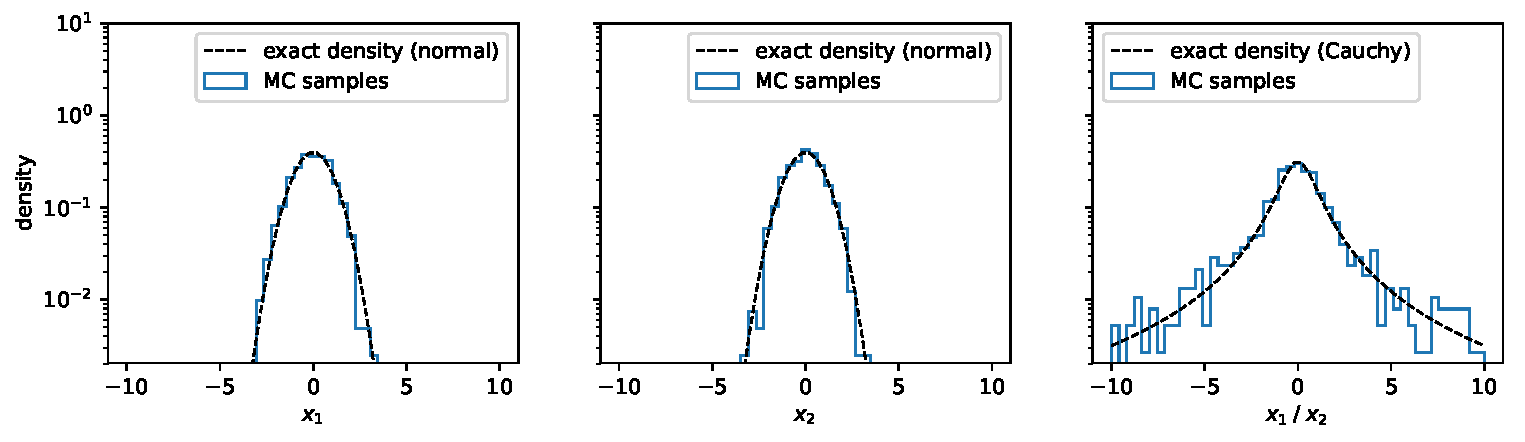
\includegraphics[width=\textwidth]{./figs/07-Cauchy.pdf}
\end{figure}

\newpage
\no {\bf Example:} Entropy of distributions from flat Dirichlet
\begin{itemize}
	\item Input: $p = (p_1, p_2, p_3) \in [0,1]^{\times 3}$, such that $\sum_{k=1}^3 p_k = 1$, where $P(p) = \text{Dirichlet}(p\;|\;\alpha = (1,1,1))$
	\item Output: $h := H(p) = -\sum_k p_k \log_2 p_k$,\; $P(h) = \;?$
	\item MC method:
\begin{lstlisting}[language=python]
import numpy as np
from scipy.stats import dirichlet

def entropy(p):
    h = 0
    for pk in p:
        if pk > 0:
            h += - pk * np.log2(pk)
    return h

alpha = (1,1,1)
sample_size = 10_000
p_samples = dirichlet.rvs(alpha, size=sample_size)
h_samples = []    
for p in p_samples:
    h_samples.append(entropy(p))
\end{lstlisting}
\end{itemize}
\begin{figure}[h]
\centering
	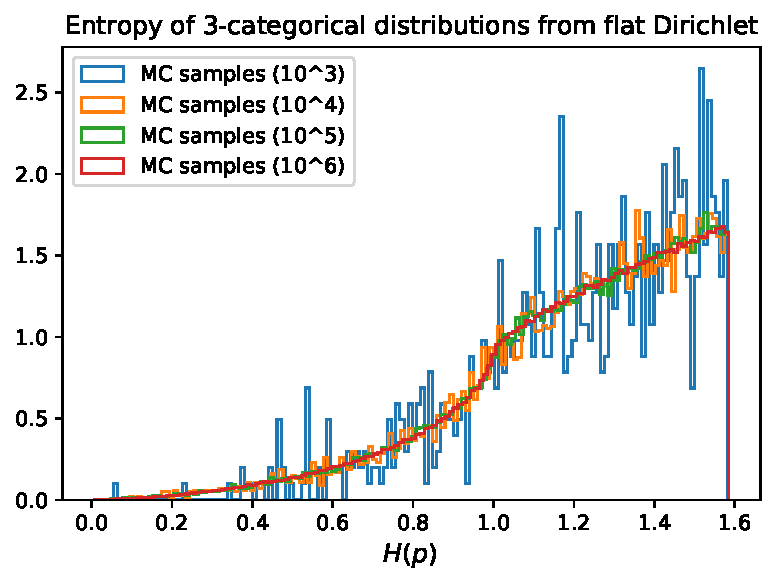
\includegraphics[width=0.7\textwidth]{./figs/07-entropy.pdf}
\end{figure}

\newpage
\no {\bf Example:} Monty Hall problem
\begin{itemize}
	\item Input: 
		\begin{itemize}
			\item In a game show, there a three doors $D = \{1,2,3\}$
			\item A reward is placed behind door $r\in D$ uniformly randomly, i.e. $P(r) = \text{uniform}$.
			\item The player picks a door $p_1 \in D$ uniformly randomly, i.e. $P(p_1) = \text{uniform}$ (He doesn't know where the reward is.)
			\item The game show master (who knows where the reward is), pick a door from the remaining two that does not have the reward, and opens it, $o \in D_\text{can open}$, where $D_\text{can open} = D \setminus (\{r\} \cup \{p_1\})$ randomly, i.e. $P(o) = \text{uniform}$.
			\item The game show master offers the player another chance to pick one of the remaining two doors $D_\text{remaining} = D \setminus \{o\}$. He can stick to his first choice, i.e. $p_2 = p_1$, or switch to the other door, i.e. $p_2 \in D_\text{remaining}\setminus \{p_1\}$
			\item The game show master opens door $p_2$, and the player wins if $p_2 = r$, and loses otherwise.
		\end{itemize}
	\item Output: What's the probability of winning with the two strategies, i.e.
	\ba
		P(\text{win}\;|\;\text{switch}) = P(r=p_2\;|\;p_2 \neq p_1) &=& ?  \\
		P(\text{win}\;|\;\text{don't switch}) = P(r=p_2\;|\;p_2 = p_1) &=& ?
	\ea
	\item MC method:
\begin{lstlisting}[language=python]
from numpy.random import choice

doors = {1, 2, 3}

games = 1000
wins_with_switch = 0
wins_with_no_switch = 0
for g in range(games):
    reward = choice(list(doors))
    pick_1 = choice(list(doors))

    can_open = doors - set([pick_1]).union(set([reward]))
    openned = choice(list(can_open))
    remaining = doors - set([openned])
    
    pick_2 = list(remaining - set([pick_1]))[0]
    if pick_2 == reward:
        wins_with_switch += 1
    
    pick_2 = pick_1
    if pick_2 == reward:
        wins_with_no_switch += 1
        
P_win_with_switch = wins_with_switch / float(games)
P_win_with_no_switch = wins_with_no_switch / float(games)
\end{lstlisting}
Yielding something similar to $P(\text{win}\;|\;\text{switch}) \approx 0.653$, and $P(\text{win}\;|\;\text{don't switch}) \approx 0.347$.

\end{itemize}

\subsection{Markov Chain Monte Carlo method}
\begin{itemize}
	\item {\bf Goal:} Draw samples from an unnormalized posterior $P\s(\theta) \mapsto \{\theta^{(s)}\}$
	\item {\bf Challenge:} We don't know how to do this directly.
	\item {\bf Method:}
	\begin{enumerate}
		\item Initialize $\theta^{(0)}$.
		\item Obtain a new $\theta^{(s+1)}$ value using the current value $\theta^{(s)}$ and the $P\s()$ function.
		\item Add the new value to the list of samples $\{\theta^{(s)}\}$. Return to step 2 with $s \leftarrow s+1$.
	\end{enumerate}
\end{itemize}
\begin{figure}[h]
\centering
	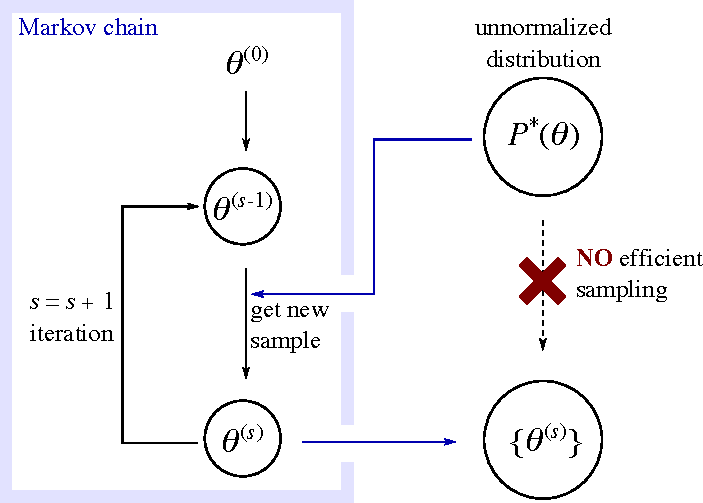
\includegraphics[width=0.5\textwidth]{./figs/07-MCMC.pdf}
\end{figure}
Various Markov chain-based methods exist: Metropolis-Hastings sampling, Gibbs sampling, Hamiltonian sampling.

\subsection{Metropolis Hastings sampling}
\begin{enumerate}
	\item Start with $\theta^{(0)}$.
	\item Propose a new value: $\theta^\text{new} = \theta^{(s)} + \varepsilon$, where $\varepsilon$ is drawn from $P(\varepsilon) = \text{Normal}(\varepsilon\;|\;0, s^2)$, where $s$ is a fixed ``step size''.
	\item Evaluate $\Delta L = \log P\s(\theta^\text{new}) - \log P\s(\theta^{(s)})$, and depending on its value, we obtain $\theta^{(s+1)}$:
	\begin{enumerate}
		\item If $\Delta L >= 0$, then 
		\be	
			\theta^{(s+1)} = \theta^\text{new},
		\ee
		\item if $\Delta L < 0$, then 
		\be
			\theta^{(s+1)} = 
			\left\{
			\begin{array}{ll}
				\theta^\text{new}& \text{with probability } \exp(\Delta L)
				\\
				\theta^{(s)} & \text{with probability } 1 - \exp(\Delta L)
			\end{array}
			\right.
		\ee
	\end{enumerate}

\newpage
\no {\bf Example:} Bimodal distribution
\begin{itemize}
	\item Unnormalized distribution: $\log P\s(x) = x / 2 - \big(1 - x^2\big)^2$, where $x \in \mathds{R}$.
	\item 1-dimensional Metropolis-Hastings sampler:
\begin{lstlisting}[language=python]
def propose_MH(x, stepsize):
    epsilon = norm.rvs(loc=0, scale=stepsize)
    return x + epsilon

def new_sample_MH(x_current, x_proposed, log_Pstar):
    delta_L = log_Pstar(x_proposed) - log_Pstar(x_current)
    if delta_L >= 0:
        return x_proposed
    if np.random.random() < np.exp(delta_L):
        return x_proposed
    else:
        return x_current
\end{lstlisting}
	\item Applying it to the $\log P\s$ in question:
\begin{lstlisting}[language=python]
def log_Pstar_camel(x):
    return 0.5 * x -(1 - x**2)**2

x0 = 0
stepsize = 0.1
iterations = 20000
x_samples = []

x_curr = x0
for it in range(iterations):
    x_proposed = propose_MH(x_curr, stepsize)
    x = new_sample_MH(x_curr, x_proposed, log_Pstar_camel)
    x_samples.append(x)
    x_curr = x
\end{lstlisting}
\end{itemize}

\begin{figure}[h]
\centering
	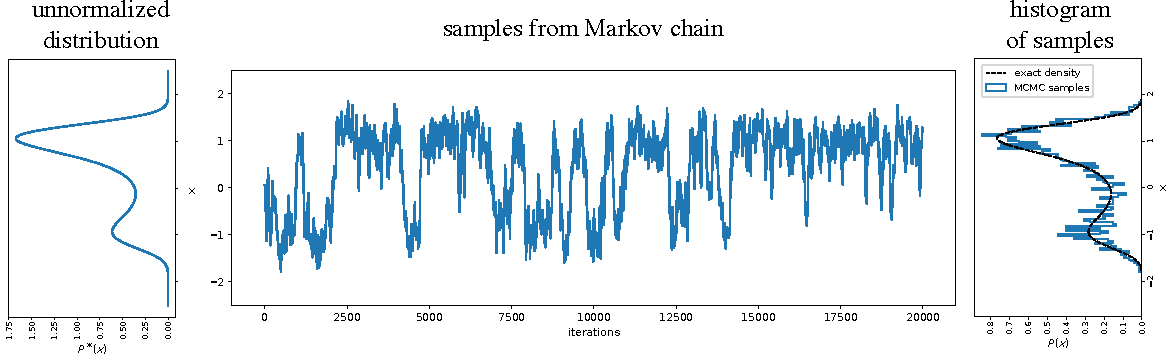
\includegraphics[width=1.1\textwidth]{./figs/07-camel-MH.pdf}
\end{figure}
\end{enumerate}







\end{document}